\section*{Abstract}

Replication studies are essential for assessing the credibility of claims from
original studies. A critical aspect of designing replication studies is
determining their sample size; a too small sample size may lead to inconclusive
studies whereas a too large sample size may waste resources that could be
allocated better in other studies. Here we show how Bayesian approaches can be
used for tackling this problem. The Bayesian framework allows researchers to
combine the original data and external knowledge in a design prior distribution
for the underlying parameters. Based on a design prior, predictions about the
replication data can be made, and the replication sample size can be chosen to
ensure a sufficiently high probability of replication success. Replication
success may be defined through Bayesian or non-Bayesian criteria, and different
criteria may also be combined to meet distinct stakeholders and allow conclusive
inferences based on multiple analysis approaches. We investigate sample size
determination in the normal-normal hierarchical model where analytical results
are available and traditional sample size determination is a special case where
the uncertainty on parameter values is not accounted for. An application to data
from a multisite replication project of social-behavioral experiments
illustrates how Bayesian approaches help to design informative and
cost-effective replication studies. Our methods can be used through the R
package \texttt{BayesRepDesign}.

\textbf{Key words}: Bayesian design, design prior, multisite replication, sample
size determination



\section{Introduction}

The replicability of research findings is a cornerstone for the credibility of
science. However, there is growing evidence that the replicability of many
scientific findings is lower than expected \citep{Ioannidis2005,Opensc2015,
  Camerer2018, Errington2021}. This ``replication crisis'' has led to
methodological reforms in various fields of science, one of which is an
increased conduct of replication studies \citep{Munafo2017}. Statistical
methodology plays a key role in the evaluation of replication studies, and
various methods have been proposed for quantifying how ``successful'' a
replication study was in replicating the original finding \citep[among
others]{Bayarri2002, Verhagen2014, Simonsohn2015, Anderson2016, Patil2016,
  Johnson2016, Etz2016, vanAert2017, Ly2018, Harms2019, Hedges2019, Mathur2020,
  Held2020, Pawel2020, Bonett2020, Held2021, Pawel2022b}. Yet, as with ordinary
studies, statistical methodology is not only important for analyzing replication
studies but also for designing them, in particular for their \emph{sample size
  determination} (SSD). Optimal SSD is important since too small sample sizes
may lead to inconclusive studies, whereas too large sample sizes may waste
resources which could have been allocated better in other research projects.

SSD for replication studies comes with unique opportunities and challenges; the
data from the original study can be used to inform SSD, at the same time the
analysis of replication success based on original and replication study is
typically different from an analysis of a single study for which traditional SSD
methodology was developed. Since analysis and design of replication studies
should be in accordance, a relatively small literature has emerged which
specifically deals with replication study power calculations and SSD
\citep{Bayarri2002, Goodman1992, Senn2002, Anderson2017, Micheloud2020,
  vanZwet2022, Held2020, Pawel2022b, Hedges2021, Anderson2022}. However, most of
these articles only deal with selected analysis methods and data models. % For
% instance, SSD for standardized mean difference effect sizes analyzed with Bayes
% factors \citep{Bayarri2002}, SSD for statistical significance assessment of the
% replication \citep{Goodman1992, Senn2002, Micheloud2020, vanZwet2022}, SSD for
% reverse-Bayes assessment of replication studies \citep{Held2020, Pawel2022b}, or
% SSD for meta-analysis of replication studies \citep{Hedges2021}.
An exception is the excellent article by \citet{Anderson2022} which discusses
more general principles of replication SSD in the context of psychological
research, mostly from a frequentist perspective. As they state ``the literature
on Bayesian sample size planning is still nascent, particularly with respect to
Bayes Factors \citep{Schoenbrodt2017}, and has not yet been clearly optimized
for the context of most replication goals'' \citep[p. 18]{Anderson2022}. Our
goal is therefore to complement their article by developing a unified framework
of replication SSD (schematically illustrated in Figure~\ref{fig3:SSDschema})
based on principles from Bayesian design approaches \citep{Spiegelhalter1986b,
  Spiegelhalter1986c, Weiss1997, OHagan2001b, Gelfand2002, DeSantis2004,
  Spiegelhalter2004, Schoenbrodt2017, Pek2019, Kunzmann2021, Park2022,
  Grieve2022}. We aim to provide both a theoretical basis for methodologists
developing new methods for design and analysis methods of replication studies,
and also to illustrate how Bayesian design approaches can practically be used by
researchers planning a replication study.

\begin{figure}[!ht]
  \centering
  \begin{tikzpicture}[thick, node distance = 11em and 1em,
  font=\fontsize{10pt}{12pt}\selectfont]

   % nodes
    \node[rectangle, draw, rounded corners = 0.2em] (oData)
    {\begin{tabular}{c} \textbf{Original data} \\
        {\scriptsize $f(x_{o} \given \theta)$} \\
     \end{tabular}};

   \node (designPrior) [below right = 3.5em and 2em of oData]
   {\begin{tabular}{c} \textbf{Design prior for model parameter} \\
      {\scriptsize $f(\theta \given x_{o}, \mathrm{external~
      knowledge})$}\\
    \end{tabular}};


  \node[rectangle, draw, rounded corners = 0.2em] (external) [right = 17em of oData]
  {\begin{tabular}{c} \textbf{Initial prior for model parameter} \\
     {\scriptsize $f(\theta \given \mathrm{external~knowledge})$} \\
   \end{tabular}};

   \node[rectangle, draw, rounded corners = 0.2em] (externalknowl) [below = 2em of external]
   {\begin{tabular}{l}
      \multicolumn{1}{c}{\textbf{External knowledge}} \\
     {\scriptsize -- between-study heterogeneity} \\
     {\scriptsize -- scepticism regarding original study} \\
     {\scriptsize -- data from other studies} \\
     {\scriptsize $\phantom{\rightarrow} \hdots$} \\
   \end{tabular}};


 \node (rData) [below = 4.5em of designPrior]
 {\begin{tabular}{c} \textbf{Predictive distribution of replication data} \\
    {\scriptsize $f(x_{r} \given n_{r}, x_{o}, \mathrm{external~
    knowledge})$}
  \end{tabular}};

\node[rectangle, draw, fill = lightlightgray] (nr) [below = 2em of externalknowl]
{\begin{tabular}{c} \textbf{Replication sample size} \\
   {\scriptsize $n_{r}$}
 \end{tabular}};


\node (PRS) [below = 4.5em of rData]
{\begin{tabular}{c} \textbf{Probability of replication success} \\
   {\scriptsize $\Pr(X_r \in S \given n_{r}, x_{o}, \mathrm{external
    knowledge})$}
 \end{tabular}};

\node[rectangle, draw, rounded corners = 0.2em] (measureRS) [below = 15em of oData]
{\begin{tabular}{c} \textbf{Analysis method}  \\
    {\scriptsize success region $S$} \\
 \end{tabular}};

\node[rectangle, draw, rounded corners = 0.2em] (sideCond) [below = 2.5em of nr]
{\begin{tabular}{l}
   \multicolumn{1}{c}{\textbf{Constraints}} \\
   {\scriptsize -- type I error rate requirements} \\
   {\scriptsize -- cost/availability constraints} \\
   {\scriptsize $\phantom{\rightarrow} \hdots$} \\
 \end{tabular}};


% edges
\draw [->] [bend left] (oData.east) to ([xshift=-1em]designPrior.north);
\draw [->] [bend right] (external.west) to ([xshift=1em]designPrior.north);
\draw [->] (designPrior) to (rData);
\draw [->] (rData) to (PRS.north);
\draw [->] [bend right] (nr.west) to ([xshift=1em]rData.north);
\draw [->] [bend left] (measureRS.east) to ([xshift=-1em]PRS.north);
\draw [->] [dashed] (oData) to (measureRS);
\draw [->] [dashed] (sideCond) to (nr.south);
\draw [->] [dashed] (externalknowl.north) to (external.south);


\end{tikzpicture}

  \caption{Schematic illustration of Bayesian sample size determination for
    replication studies. The original and replication data are denoted by
    $x_{o}$ and $x_{r}$, respectively. Both are assumed to come from a
    distribution with density/probability mass function denoted by
    $f(x_{i} \given \theta)$ for $i \in \{o, r\}$. An initial prior with density
    function $f(\theta \given \mathrm{external~knowledge})$ is assigned to the
    model parameter $\theta$.}
\label{fig3:SSDschema}
\end{figure}

The design of replication studies is a natural candidate for Bayesian knowledge
updating as it allows to combine uncertain information from different sources
--for instance, the data from the original study and/or expert knowledge-- in a
so-called \emph{design prior} distribution for the underlying model parameters.
If the analysis of the replication data is also Bayesian, the design prior may
be different from the so-called \emph{analysis prior} which, unlike the design
prior, is usually desired to be objective or ``uninformative''
\citep{OHagan2001b}. Based on the design prior, predictions about the
replication data can then be made, and the sample size can be chosen such that
the probability of replication success becomes sufficiently high. Importantly,
Bayesian design approaches can also be used if the planned analysis of the
replication study is non-Bayesian, which is the more common situation in
practice. Bayesian design based on a frequentist analysis is known under various
names, such as ``hybrid classical-Bayesian design'' \citep{Spiegelhalter2004} or
``Bayesian assurance'' \citep{OHagan2005}, and has also been used before for
psychological applications \citep{Pek2019, Park2022} and replication studies
\citep{Anderson2017, Micheloud2020}.

This paper is structured as follows: We start with presenting a general
framework for Bayesian SSD of replication studies which applies to any kind of
data model and analysis method. We then investigate design priors and SSD in the
normal-normal hierarchical model framework which provides sufficient flexibility
for incorporating the original data and external knowledge in replication
design. No advanced computational methods, such as (Markov Chain) Monte Carlo
sampling, are required for conducting Bayesian SSD in this framework, and in
many cases there are even simple formulae which generalize classical power and
sample size calculations. We illustrate the methodology for several Bayesian and
non-Bayesian analysis methods, and for both singlesite and multisite replication
studies. Since multisite replication studies are becoming increasingly popular
in psychology \citep[\eg{}][]{Klein2018}, we also discuss how to choose the
optimum allocation of samples within and between sites from a Bayesian design
point of view. As a running example we use data from a multisite replication
project of social-behavioral experiments \citep{Protzko2020}. Finally, we close
with concluding remarks, limitations, and open questions.



\section{General framework} \label{sec3:GFW}

% Figure~\ref{fig3:SSDschema} schematically illustrates the process of Bayesian SSD
% for replication studies, which we will explain in more detail in the following.
Suppose an original study has been conducted and resulted in a data set $x_{o}$.
These data are assumed to come from a distribution characterized by an unknown
parameter $\theta$ and with density function $f(x_{o} \given \theta)$. To assess
the replicability of a claim from the original study, an independent and
identically designed (apart from the sample size) replication study is
conducted, and the goal of the design stage is to determine its sample size
$n_{r}$.

As the observed original data $x_{o}$, the yet unobserved replication data
$X_{r}$ are assumed to come from a distribution depending on the parameter
$\theta$. The parameter $\theta$ thus provides a link between the two studies,
and the knowledge obtained from the original study can be used to make
predictions about the replication. The central quantity for doing so is the
so-called \emph{design prior} of the parameter $\theta$, which we write as the
posterior distribution of $\theta$ based on the original data and an
\emph{initial prior} for $\theta$
\begin{align}
  \label{eq3:dp}
  f(\theta \given x_o, \mathrm{external~knowledge}) =
  \frac{f(x_o \given \theta) \, f(\theta \given \mathrm{external~knowledge})}{f(x_o \given
  \mathrm{external~knowledge})}.
\end{align}
The initial prior of $\theta$ may depend on external knowledge (\eg{} data from
other studies) and it represents the uncertainty about $\theta$ before observing
the original data. We will discuss common types of external knowledge in the
replication setting in the next Section. %~\ref{sec3:SS}.
The design prior~\eqref{eq3:dp} hence represents the state of knowledge and
uncertainty about the parameter $\theta$ before the replication is conducted,
and, along with an assumed replication sample size $n_{r}$, it can be used to
compute a predictive distribution for the replication data
\begin{align}
  \label{eq3:ftr}
  f(x_r \given n_r, x_o, \mathrm{external~knowledge})
  &= \int%_\Theta
  % \underbrace{f(x_r \given n_{r}, \theta)}_{\mathrm{likelihood}}
    f(x_r \given n_{r}, \theta)
    % \, \underbrace{f(\theta \given x_o, \mathrm{external~knowledge})}_{\mathrm{design prior}}
    \, f(\theta \given x_o, \mathrm{external~knowledge})
    \, \mathrm{d}\theta.
\end{align}

After completion of the replication, the observed data $x_r$ will be analyzed in
some way to quantify to what extent the original result could be replicated. The
analysis may involve the original data (for example, a meta-analysis of the two
data sets) or it may only use the replication data. Typically, there is a
\emph{success region} $S$ which implies that if the replication data fall within
it ($x_r \in S$), the replication is successful. The \emph{probability of
  replication success} can thus be computed by integrating the predictive
density~\eqref{eq3:ftr} over $S$. To ensure a sufficiently conclusive replication
design, the sample size $n_{r}$ is determined such that the probability of
replication success is at least as large as a desired target probability of
success, here and henceforth denoted by $1 - \beta$. The required sample size
$n_r^*$ is then the smallest sample size which leads to a probability of
replication success of at least $1 - \beta$, \ie{}
\begin{align}
  \label{eq3:nr}
  n_r^* = \inf \left\{n_r : \Pr(X_{r} \in S \given
  n_r, x_{o}, \mathrm{external~knowledge}) \geq 1 - \beta \right\}.
\end{align}

Often, replication studies are analyzed using several methods which quantify
different aspects of replicability, and which have different success regions
(\eg{} one method for quantifying parameter compatibility and another for
quantifying evidence against a null hypothesis). In this case, the sample size
may be chosen such that the probability of replication success is as large as
desired for all planned analysis methods.

There may sometimes be certain constraints which the replication sample size
needs to satisfy. For instance, in most cases there is an upper limit on the
possible sample size due to limited resources and/or availability of samples.
Moreover, funders and regulators may also require methods to be
\emph{calibrated} \citep{Grieve2016}, that is, to have appropriate type I error
rate control. The sample size $n_r^*$ may thus also need to satisfy a type I
error rate not larger than some required level.
% Similarly, it may be reasonable to have \emph{precision} constraints, \eg{} to
% require that a confidence interval for the replication effect estimate has to be
% at least as tight as the confidence interval estimated in the original study.






\section{Sample size determination in the normal-normal hierarchical model}
\label{sec3:SS}
We will now illustrate the general methodology from the previous section in the
\emph{normal-normal hierarchical model} where predictive distributions and the
probability of replication success can often be expressed in closed-form,
permitting further insight. % To conduct SSD for replication studies
It is pragmatic to adopt a meta-analytic perspective and use only study level
summary statistics instead of the raw study data since the raw data from the
original study are not always available to the replicators. Typically, the
underlying parameter $\theta$ is a univariate effect size quantifying the effect
on the outcome variable (\eg{} a mean difference, a log odds ratio, or a log
hazard ratio). The original and replication study can then be summarized through
an effect estimate $\that$, possibly the maximum likelihood estimate, and a
corresponding standard error $\sigma$, \ie{} $x_{o} = \{\that_{o}, \sigma_{o}\}$
and $x_{r} = \{\that_{r}, \sigma_{r}\}$. Effect estimates and standard errors
are routinely reported in research articles or can, under some assumptions, be
computed from $p$-values and confidence intervals. As in the conventional
meta-analytic framework \citep{Sutton2001}, we further assume that for study
$k \in \{o, r\}$ the (suitably transformed) effect estimate $\hat{\theta}_k$ is
approximately normally distributed around a study specific effect size
$\theta_k$ and with (known) variance equal to its squared standard error
$\sigma_k^2$, here and henceforth denoted by
$\hat{\theta}_k \given \theta_k \sim \Nor(\theta_k, \sigma_k^2)$. The standard
error $\sigma_k$ is typically of the form $\sigma_k = \lambda/\sqrt{n_k}$ with
$\lambda^{2}$ some unit variance and $n_{k}$ the sample size. The ratio of the
original to the replication variance is thus the ratio of the replication to the
original sample size
\begin{align*}
  c = \sigma^2_o/\sigma^2_r = n_r/n_o,
\end{align*}
which is often the main focus of SSD as it quantifies how much the replication
sample $n_{r}$ size needs to be changed compared to the original sample size
$n_{o}$. Depending on the effect size type, this framework might require slight
modifications \citep[see \eg{}][chapter 2.4]{Spiegelhalter2004}.

Assuming a normal sampling model for the effect
estimates~\eqref{eq3:hat_theta_k}, as described previously, and specifying an
initial hierarchical normal prior for the study specific effect
sizes~\eqref{eq3:theta_k} and the effect size~\eqref{eq3:theta}, leads then to the
normal-normal hierarchical model
\begin{subequations}
\label{eq3:hierarch-model}
\begin{align}
  \hat{\theta}_k \given \mspace{-1mu} \theta_k &\sim \Nor(\theta_k, \sigma_k^2)
  \label{eq3:hat_theta_k} \\
  \theta_k \given \theta \,\,  &\sim \Nor(\theta, \tau^2) \label{eq3:theta_k} \\
  \theta \,\, &\sim \Nor(\mutheta,
  \sigmatheta^2). \label{eq3:theta}
\end{align}
\end{subequations}
By marginalizing over the study specific effects sizes, the
model~\eqref{eq3:hierarch-model} can alternatively be expressed as
\begin{subequations}
\label{eq3:hierarch-model2}
\begin{align}
  \hat{\theta}_k \given \mspace{-1mu} \theta &\sim \Nor(\theta, \sigma_k^2 + \tau^{2})
  \label{eq3:hat_theta_k2} \\
  \theta  &\sim \Nor(\mutheta,
  \sigmatheta^2) \label{eq3:theta2}
\end{align}
\end{subequations}
which is often more useful for derivations and computations. In the following we
will explain how the normal-normal hierarchical model can be used
% is similar to the random effects model typically used in meta-analysis, and
% to incorporate the original data and external knowledge into
for SSD of the replication study.

\subsection{Design prior and predictive distribution}
\label{sec3:designpredictive}
The observed original data $x_{o} = \{\that_{o}, \sigma_{o}\}$ can be combined
with the initial prior~\eqref{eq3:theta2} %by Bayes' theorem~\eqref{eq3:dp}
by standard Bayesian theory for normal prior and likelihood \citep[ch.
3.7]{Spiegelhalter2004} to obtain a posterior distribution for the effect size
$\theta$
\begin{align}
  \label{eq3:dpnormal}
  \theta \given \hat{\theta}_o, \sigma^2_o
  \sim
  \Nor\left(
  \frac{\hat{\theta}_o}{1 + 1/g} + \frac{\mutheta}{1 + g},
  \frac{\sigma^2_o + \tau^2}{1 + 1/g} \right)
\end{align}
where $g = \sigmatheta^2/(\sigma^2_o + \tau^2)$ is the \emph{relative prior
  variance}. This posterior serves then as the design prior for predicting the
replication data.

It is interesting to contrast the design prior \eqref{eq3:dpnormal} to the
``conditional'' design prior \citep{Micheloud2020}, that is, to assume that the
unknown effect size $\theta$ corresponds to the original effect estimate
$\that_{o}$. This is a standard approach in practice, for instance,
\citet{Opensc2015} determined the sample sizes of its 100 replications under
this assumption. In our framework it implies that the normal design
prior~\eqref{eq3:dpnormal} becomes a point mass at the original effect estimate
$\that_{o}$, which can either be achieved through overwhelmingly informative
original data ($\sigma^{2}_{o} \downarrow 0$) along with no heterogeneity
($\tau^{2} = 0$), or through an overwhelmingly informative initial prior
($g \downarrow 0$) centered around the original effect estimate
($\mutheta = \that_{o}$). Both cases show that from a Bayesian perspective the
standard approach is unnatural as it either corresponds to making the standard
error $\sigma_{o}$ smaller than it actually was, or to cherry-picking the prior
based on the data.


Based on the design prior~\eqref{eq3:dpnormal}, the predictive distribution of
the replication effect estimate $\that_{r}$ can then be computed by assuming a
replication standard error $\sigma_{r}$ and integrating the marginal density of
the replication effect estimate~\eqref{eq3:hat_theta_k2} with respect to the
prior density, leading to
\begin{align}
  \label{eq3:fthetar}
  \hat{\theta}_r \given \hat{\theta}_o, \sigma^2_o, \sigma^2_r
  \sim
  \Nor\left(\muthatr =
  \frac{\hat{\theta}_o}{1 + 1/g} + \frac{\mutheta}{1 + g}, \sigmathatr^{2} =
  \, \sigma^2_r + \tau^2 + \frac{\sigma^2_o + \tau^2}{1 + 1/g}\right)
\end{align}
which can again be shown using standard Bayesian theory \citep[ch.
3.13.3]{Spiegelhalter2004}.
% For some analysis methods, replication success is more naturally defined via the
% replication $z$-value $z_{r} = \that_{r}/\sigma_{r}$. In these cases, it can be
% more convenient to use the associated predictive distribution of $z_{r}$
% \begin{align}
%   \label{eq3:zr}
%   z_r \given z_o, c%,  z_{\scriptscriptstyle{\theta}},h, g
%   \sim
%   \Nor\left\{\muzr =
%   \sqrt{c} \left(\frac{z_o}{1 + 1/g} +
%   \frac{z_{\scriptscriptstyle{\theta}} \sqrt{g  (1 + h)}}{1 + g}\right),
%   \sigmazr^{2} =
%   \, 1 + c \left( h + \frac{1 + h}{1 + 1/g}  \right) \right\}
% \end{align}
% which only depends on relative parameters, \ie{} the variance ratio
% $c = \sigma^{2}_{o}/\sigma^{2}_{r}$, the original $z$-value
% $z_{o} = \that_{o}/\sigma_{o}$, the prior $z$-value
% $z_{\scriptscriptstyle{\theta}} = \mutheta/\sigma_{\scriptscriptstyle{\theta}}$,
% and the relative heterogeneity $h = \tau^{2}/\sigma^{2}_{o}$.
The design prior~\eqref{eq3:dpnormal} and the resulting predictive
distribution~\eqref{eq3:fthetar}
% and~\eqref{eq3:zr}
depend on the parameters of the initial prior ($\tau^ {2}$, $\mutheta$,
$\sigmatheta^{2}$). We will now explain how these parameters can be specified
based on external knowledge.

\subsection{Incorporating external knowledge in the initial prior}
\label{sec3:initialPrior}

At least three common types of external knowledge can be distinguished in the
replication setting: (i) expected heterogeneity between original and replication
study due to differences in study design, execution, and population, (ii) prior
knowledge about the effect size either from theory or from related studies,
(iii) scepticism regarding the original study due to the possibility of
exaggerated results.



\subsubsection{Between-study heterogeneity}
\label{sec3:heterogeneity}
The expected degree of between-study heterogeneity can be incorporated via the
variance $\tau^2$ in~\eqref{eq3:theta_k}. As $\tau^{2}$ decreases, the study
specific effect sizes become more similar, whereas for increasing $\tau^{2}$
they become more unrelated. If the replicators do not expect any heterogeneity
they can thus set $\tau^{2} = 0$ which will lead to the model collapsing to a
fixed effects model.

If heterogeneity is expected, there are different approaches for specifying
$\tau^{2}$. A domain expert may subjectively assess how much heterogeneity is to
be expected due to the change in laboratory, study population, and other
factors. An alternative is to take an estimate from the literature, \eg{} from
multisite replication projects or from systematic reviews. Finally, one can also
specify an upper limit of ``tolerable heterogeneity''. This approach is similar
to specifying a minimal clinically relevant difference in classical power
analysis in the sense that a true replication effect size which is intolerably
heterogeneous from the original effect size is not relevant to be detected. An
absolute \citep[chapter 5.7.3]{Spiegelhalter2004} and a relative approach
\citep{Held2020c} can be considered. In the absolute approach, a value of
$\tau^{2}$ is chosen such that a suitable range of study-specific effect sizes
is not larger than an effect size difference considered negligible. For example,
when 95\% of the study specific effect sizes should not vary more than a small
effect size \eg{} $d = 0.2$ on standardized mean difference
scale based on the \citet{Cohen1992} effect size classification, this would lead
to $\tau = d/(2 \cdot 1.96) \approx 0.05$. % Similarly, one
% could consider the distribution of the difference of two effect sizes
% $\theta_{1} - \theta_{2} \given \theta \sim \Nor(0, 2\tau^{2})$ and choose
% $\tau$ such that the, \eg{} the 95\% range is not larger than some desired
% value.
In the relative approach, $\tau^{2}$ is specified relative to the variance of
the original estimate $\sigma^{2}_{o}$ using field conventions for tolerable
relative heterogeneity. For example, in the Cochrane guidelines for systematic
reviews \citep{Deeks2019} a value of
$I^{2} = \tau^{2}/(\tau^{2} + \sigma^{2}_{o}) = 40\%$ is classified as
``negligible'', which translates to
$\tau^{2} = \sigma^{2}_{o}/(1/I^{2} - 1) = (2\sigma^{2}_{o})/3$.

We note that one can also assign a prior distribution to $\tau^2$ \citep[for an
overview of prior distributions for heterogeneity variances in the normal-normal
hierarchical model see][]{Rover2021}. In this case there is no closed-form
expression for the predictive distribution of the replication effect estimate
but numerical or Monte Carlo integration need to be used. % To
% gain more insight, we will thus only consider fixed $\tau^{2}$ in the remaining
% part of the paper.
We illustrate in the supplement how the probability of replication success can
in this case be computed. The derived closed-form expressions conditional on
$\tau^{2}$ are still useful as they enable computation of the predictive
distribution up to a single one-dimensional integral which can be computed
numerically.
% However, a relatively straightforward solution is to first simulate from the
% marginal posterior distribution of $\tau^{2}$ based on an the original data
% $x_{o} = \{\that_{o}, \sigma_{o}\}$ and initial prior for $\theta$ and
% $\tau^{2}$, and then compute the relevant quantity based on the closed-form
% expression conditional on $\tau^{2}$.

\subsubsection{Knowledge about the effect size}
Prior knowledge about the effect size $\theta$ can be incorporated via the prior
mean $\mutheta$ and the prior variance $\sigmatheta^2$ in~\eqref{eq3:theta}. For
instance, the parameters may be specified based on a meta-analysis of related
studies \citep{McKinney2021} or based on expert elicitation \citep{OHagan2019}.
The resulting design prior will then contain more information than what was
provided by the original data alone, leading to potentially more efficient
designs. If there is no prior knowledge available, a standard approach is to
specify an (improper) flat prior by letting the variance go to infinity
($\sigmatheta^2 \to \infty$). The resulting design prior will then only contain
the information from the original study.

\subsubsection{Exaggerated original results}
\label{sec3:shrinkage}
Potentially exaggerated original results can be counteracted by setting
$\mutheta = 0$ which shrinks the design prior towards smaller effect sizes (in
absolute value) than the observed effect estimate $\that_{o}$. For instance,
replicators could believe that the results from the original study are
exaggerated because there is no pre-registered study protocol available. Even
without such beliefs, weakly informative shrinkage priors may also be motivated
from a ``regularization'' point of view as they can correct for statistical
biases \citep{Copas1983, Firth1993} or prevent unreasonable parameter values
from taking over the posterior in settings with uninformative data
\citep{Gelman2009}.

The amount of shrinkage is determined via the prior variance $\sigmatheta^2$. A
diffuse prior ($\sigmatheta^2 \to \infty$) will lead to no shrinkage, while a
highly concentrated prior ($\sigmatheta^2 \downarrow 0$) will completely shrink
the design prior to a point mass on zero. One option for specifying
$\sigmatheta^2$ is to use an estimate from a corpus of related studies. For
instance, \citet{vanZwet2021} used the Cochrane library of systematic reviews to
specify design priors for hypothetical replication studies of RCTs. If no corpus
is available, a pragmatic alternative is to use the empirical Bayes estimate
based on the original data
\begin{align}
  \label{eq3:EBestimate}
  \hat{\sigma}^2_{\scriptscriptstyle{\theta}} = \max\{(\that_{o} - \mutheta)^{2} - \tau^{2} - \sigma^{2}_{o}, 0\}.
\end{align}
The estimate~\eqref{eq3:EBestimate} will lead to adaptive shrinkage
\citep{Pawel2020} in the sense that shrinkage is large for unconvincing original
studies (those with small effect estimates in absolute value $|\that_{o}|$
and/or large standard errors $\sigma_{o}$), but disappears as the data become
more convincing (through larger effect estimates in absolute value $|\that_{o}|$
and/or smaller standard errors $\sigma_{o}$).




\subsection{Example: Cross-laboratory replication project}
\label{sec3:example}
We will now illustrate the construction of design priors based on data from a
recently conducted replication project \citep{Protzko2020}, see
Figure~\ref{fig3:data} for a summary of the data. The data were collected in four
laboratories which, over the course of five years, conducted their typical
social-behavioral experiments on topics such as psychology, communication, or
political science. From the experiments conducted in this period, each lab
submitted four original findings to be replicated. For instance, the original
finding from the ``Labels'' experiment was: ``When a researcher uses a label to
describe people who hold a certain opinion, he or she is interpreted as
disagreeing with those attributes when a negative label is used and agreeing
with those attributes when a positive label is used'' \citep[p.
17]{Protzko2020}, which was based on an effect estimate
$\that_{o} = 0.205$ with 95\% confidence interval from
$0.11$ to $0.3$. For each submitted
original finding, four replication studies were then carried out, one by the
same lab (a \emph{self-replication}) and three by the other three labs (three
\emph{external-replications}).

\begin{figure}[!htb]
\begin{knitrout}
\definecolor{shadecolor}{rgb}{0.969, 0.969, 0.969}\color{fgcolor}
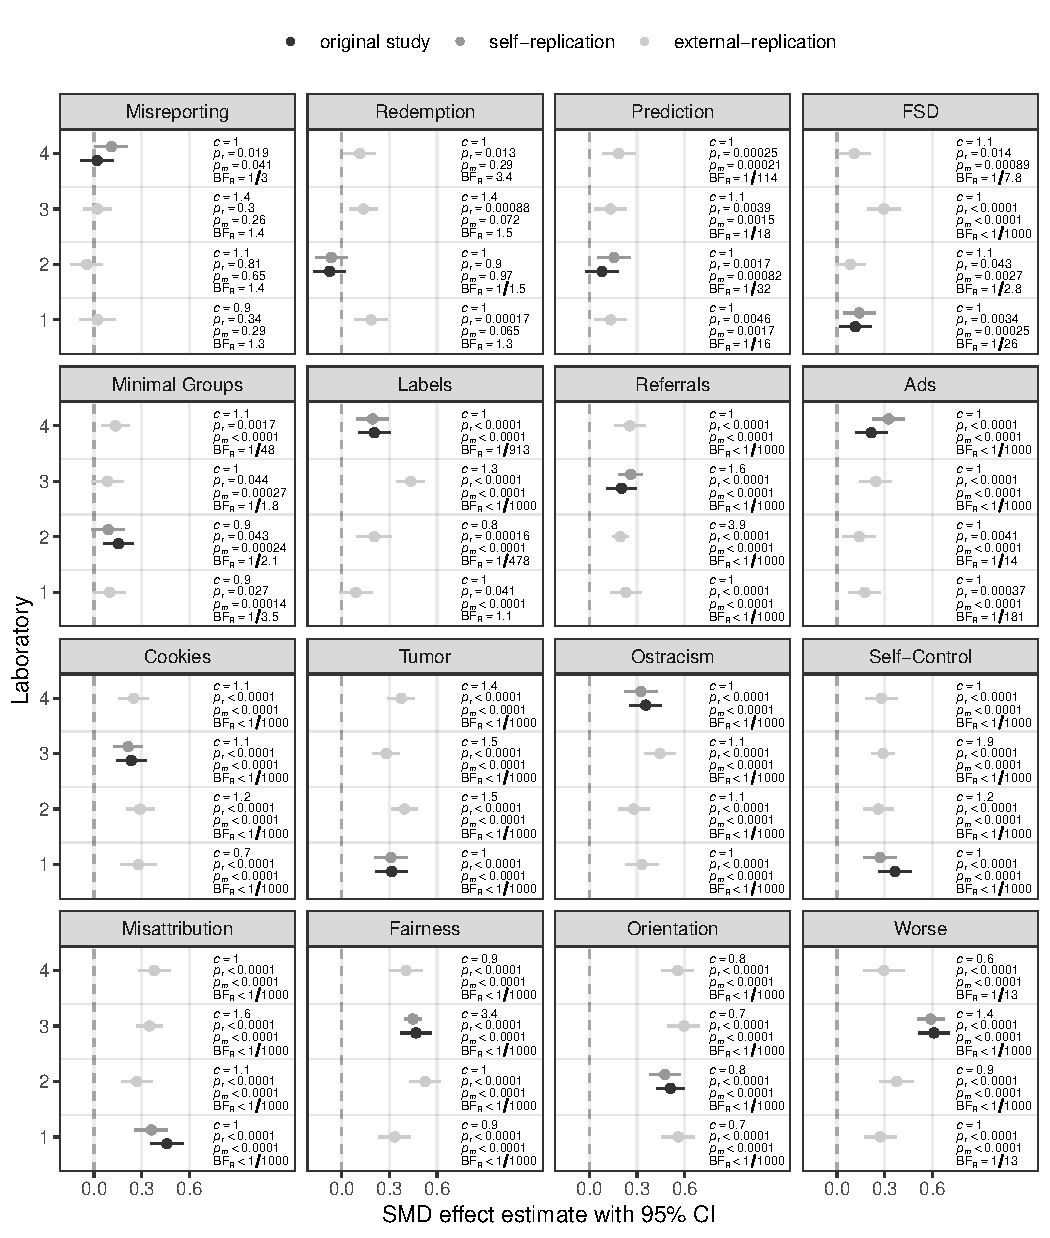
\includegraphics[width=0.97\textwidth]{images/paper3/analysis-protzko-1}
\end{knitrout}
\caption{Data from cross-laboratory replication project by \citet{Protzko2020}.
  Shown are standardized mean difference (SMD) effect estimates with 95\%
  confidence intervals stratified by experiment and laboratory. For each
  replication study, the relative sample size $c = n_{r}/n_{o}$, the one-sided
  replication $p$-value $p_{r}$, the one-sided meta-analytic $p$-value $p_{m}$,
  and the replication Bayes factor $\BFr$ are shown. Experiments are ordered
  (left to right, top to bottom) by their original one-sided $p$-value
  $p_{o} = 1 - \Phi(|\hat{\theta}_{o}|/\sigma_{o}$)}
\label{fig3:data}
\end{figure}


Most studies used simple between-subject designs with two groups and a
continuous outcome so that for a study $i \in \{o, r\}$ the standardized mean
difference (SMD) effect estimate $\that_{i}$ can be computed from the group
means $\bar{y}_{i1}, \bar{y}_{i2}$, group standard deviations $s_{i1}, s_{i2}$,
and group sample sizes $n_{i1}, n_{i2}$ by
\begin{align*}
  \that_{i} = \frac{\bar{y}_{i1} - \bar{y}_{i2}}{s_{i}}
\end{align*}
with
$s^{2}_{i} = \{(n_{i1} - 1)s_{i1}^{2} + (n_{i2} - 1)s_{i2}^{2}\}/(n_{i1} + n_{i2} - 2)$
the pooled sample variance. Under a normal sampling model and assuming equal
variances in both groups, the approximate variance of $\that_{i}$ is
\begin{align}
  \sigma^{2}_{i} = \frac{n_{i1} + n_{i2}}{n_{i1}n_{i2}} + \frac{\that_{i}^{2}}{2(n_{i1} + n_{i2})}
  \label{eq3:varSMD}
\end{align}
\citep{Hedges1981}. A cruder, but for SSD more useful, approximation
$\sigma^{2}_{i} \approx 4/n_{i}$ is obtained by assuming the same sample size in
both groups $n_{i1} = n_{i2} = n_{i}/2$, with $n_{i}$ the total sample size, and
neglecting the second term in~\eqref{eq3:varSMD} which will be close to zero for
small effect estimates and/or large sample sizes \citep{Hedges2021}. We thus
have the approximate unit variance $\lambda^{2} = 4$ and the relative variance
$c = \sigma^{2}_{o}/\sigma^{2}_{r} = n_{r}/n_{o}$,
which can be interpreted as the ratio of the replication to the original sample
size.


Suppose now the original studies have been finished, and we want to conduct SSD
for the not yet conducted replication studies. We start by specifying the design
priors (one for each replication). Since the original studies have been
preregistered, we do not expect an exaggeration of their effect estimates due to
selective reporting or other questionable research practices. Therefore, we
choose an uninformative initial prior ($\sigmatheta^{2} \to \infty$), which
leads to design prior and predictive distribution both centered around the
original effect estimate $\that_{o}$.

For specifying the between-study heterogeneity variance $\tau^{2}$, a
distinction needs to be made between self-replications and
external-replications. For self-replications it is reasonable to set
$\tau^{2} = 0$ because we would expect no between-study heterogeneity as the
experimental conditions will be nearly identical in both studies. In contrast,
one would expect some between-study heterogeneity for external-replications as
the experimental conditions may slightly differ between the labs. In the
following, we will use $\tau^{2} = 0.05^{2}$ elicited via
the ``absolute'' approach as discussed previously,
% in Section~\ref{sec3:heterogeneity},
so that the range between the 2.5\% and the 97.5\% quantile of the study
specific effect size distribution is equal to a small effect size $d = 0.2$.
% since it is independent of the sample size of the original study.

\begin{figure}[!ht]
\begin{knitrout}
\definecolor{shadecolor}{rgb}{0.969, 0.969, 0.969}\color{fgcolor}
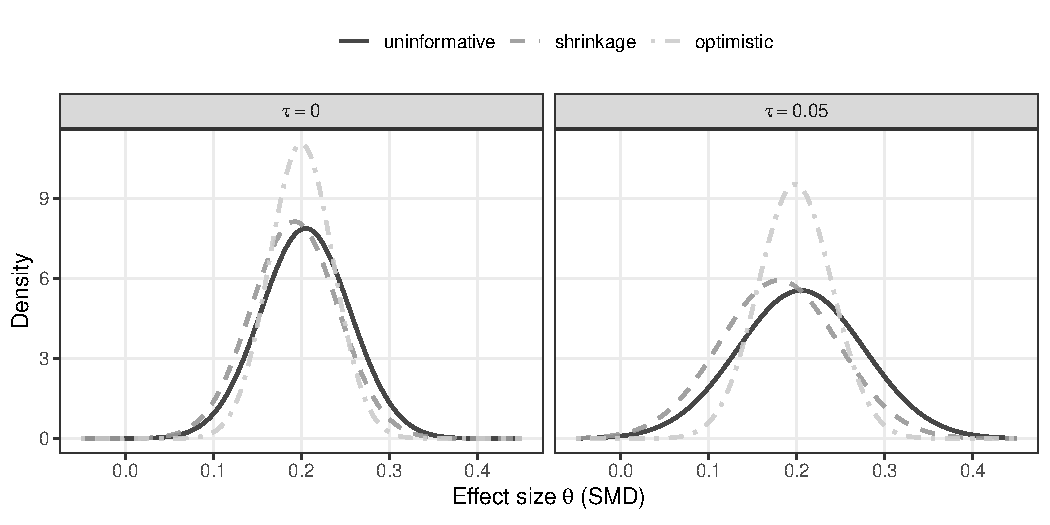
\includegraphics[width=\textwidth]{images/paper3/example-design-prior-1}
\end{knitrout}

\caption{Design priors for the effect size $\theta$ (SMD) in the experiment
  ``Labels'' based on the original effect estimate
  $\hat{\theta}_{o} = 0.205$ with standard error
  $\sigma_{o} = 0.051$. Shown are different
  choices for the between-study heterogeneity $\tau$ and the initial prior for
  the effect size $\theta$, ``uninformative'' corresponds to a flat prior,
  ``shrinkage'' corresponds to a zero-mean normal prior with empirical Bayes
  variance estimate~\eqref{eq3:EBestimate}, and ``optimistic'' corresponds to a
  flat prior updated by the data from a pilot study with effect estimate
  $\hat{\theta}_{p} = 0.195$ and standard error
  $\sigma_{p} = 0.052$.}
\label{fig3:dpexample}
\end{figure}



Taken together, we obtain the design prior
$\theta \given \hat{\theta}_{o}, \sigma^{2}_{o} \sim \Nor(\hat{\theta}_{o}, \sigma^{2}_{o})$
for self-replications and the design prior
$\theta \given \hat{\theta}_{o}, \sigma^{2}_{o} \sim \Nor(\hat{\theta}_{o}, \sigma^{2}_{o} + \tau^{2})$
with $\tau^{2} = 0.05^{2}$ for external-replications. For
example, for the experiment ``Labels'', the design prior would be
centered around the original effect estimate
$\hat{\theta}_{o} = 0.205$ with variance
$\sigma^{2}_{o} = 0.05^{2}$ for a
self-replication, and with variance
\mbox{$\sigma^{2}_{o} + \tau^{2} = 0.05^{2} + 0.05^{2} \approx 0.07^{2}$}
for an external-replication. Figure~\ref{fig3:dpexample} (dark-gray solid lines)
shows the densities of the two priors.
% Note that power
% calculations under the former prior have been termed ``predictive power''
% \citep{Micheloud2020}, while the latter prior has not appeared in the SSD for
% replication studies literature.

While these two priors seem sensible for the \citet{Protzko2020} data, it is
interesting to think about alternative scenarios. If there had been reasons to
believe that the original result might be exaggerated, we could have specified
an initial shrinkage prior ($\mutheta = 0$ and $\sigmatheta^{2} < \infty$). For
instance, the empirical Bayes estimate for the prior variance $\sigmatheta^{2}$
from~\eqref{eq3:EBestimate} leads to a prior whose mean and variance are shrunken
towards zero by $12$\% (medium-gray
dashed lines in Figure~\ref{fig3:dpexample}). In contrast, if we had prior
knowledge about the effect size $\theta$ from another study, we could have
specified an initial ``optimistic'' prior. For example, if the self-replication
of the ``Labels'' experiment had been a pilot study and we used its
effect estimate $\hat{\theta}_{p} = 0.195$ and
standard error $\sigma_{p} = 0.05$ to specify
the initial prior, this would lead to a design prior centered around the
weighted mean of original and pilot study, and a prior precision equal to the
sum of the precision of both estimates (light-gray dot-dashed lines in
Figure~\ref{fig3:dpexample}). Due to the inclusion of the external data, this
design prior is much more concentrated than the other two.


\subsection{Probability of replication success and required sample size}
To compute the probability of replication success one needs to select an
analysis method and integrate the predictive distribution~\eqref{eq3:fthetar}
% , respectively, \eqref{eq3:zr}
over the associated success region $S$. There is no universally accepted method
for quantifying replicability and here we do not intend to contribute to the
debate about the most appropriate method. We will simply show the success
regions of different methods, and how the replication sample size can be
computed from them. Some methods depend on the direction of the original effect
estimate $\that_{o}$ and throughout we will assume that it was positive
($\that_{o} > 0$). Functions for computing the probability of replication
success and the required sample size are implemented in the R package
\texttt{BayesRepDesign} (see Appendix~\ref{app3:package}) for all analysis
methods discussed in the following.


\subsubsection{The two-trials rule}
The most common approach for the analysis of replication studies is to declare
replication success when both the original and replication study lead to a
$p$-value for testing the null hypothesis $H_{0} \colon \theta = 0$ smaller than
a pre-specified threshold $\alpha$, usually $\alpha = 5\%$ for two-sided tests
and $\alpha = 2.5\%$ for one-sided tests. This procedure is known as the
\emph{two-trials rule} in drug regulation \citep{Senn2008}.

We now assume that the one-sided original $p$-value was significant at some
level $\alpha$, \ie{}
\mbox{$p_{o} = 1 - \Phi(\that_{o}/\sigma_{o}) \leq \alpha$}. Replication success
at level $\alpha$ % with the two-trials
is then achieved if the replication \mbox{$p$-value} is also significant, \ie{}
$p_{r} = 1 - \Phi(\that_{r}/\sigma_{r}) \leq \alpha$, which implies a success
region
\begin{align*}
  S_{\scriptscriptstyle \mathrm{2TR}}
  = \left[\zalpha\, \sigma_{r}, \infty \right),
\end{align*}
where $\zalpha$ is the $1 - \alpha$ quantile of the standard
normal distribution. The probability of replication success is thus given by
\begin{align}
  \label{eq3:2TRpros}
  \Pr(\that_{r} \in S_{\scriptscriptstyle \mathrm{2TR}} \given \that_{o}, \sigma_{o}, \sigma_{r})
  = % \Phi\left(\frac{\muthatr - \zalpha \, \sigma_{r}}{\sqrt{\sigma^{2}_{r} +
  % \tau^{2} + (\sigma^{2}_{o} + \tau^{2})/(1 + 1/g)}}\right)
  \Phi\left(\frac{\muthatr - \zalpha \, \sigma_{r}}{\sigmathatr}\right)
\end{align}
with $\Phi(\cdot)$ the standard normal cumulative distribution function and
$\muthatr$ and $\sigmathatr$ the mean and standard deviation of the predictive
distribution~\eqref{eq3:fthetar}. %, the latter also depending on $\sigma_{r}$.
Importantly, by decreasing the standard error $\sigma_{r}$ (through increasing
the sample size $n_{r}$), the probability of replication
success~\eqref{eq3:2TRpros} cannot become arbitrarily large but is bounded from
above by
\begin{align}
  \label{eq3:limP2TR}
  \mathrm{limPr}_{\scriptscriptstyle \mathrm{2TR}} =
  \Phi\left(\frac{ \muthatr}{\sqrt{
\tau^{2} + (\sigma^{2}_{o} + \tau^{2})/(1 + 1/g)}}\right).
\end{align}
The required replication standard error $\sigma_{r}^{*}$ to achieve a target
probability of replication success
$1 - \beta < \mathrm{limPr}_{\scriptscriptstyle \mathrm{2TR}}$ can now be obtained
by equating~\eqref{eq3:2TRpros} to $1 - \beta$ and solving for $\sigma_{r}$. This
leads to
\begin{align}
  \label{eq3:ssd2tr}
  \sigma_{r}^{*} =
  \frac{\muthatr \zalpha - \zbeta\sqrt{
  (\zalpha^{2} - \zbeta^{2})\left\{\tau^{2} + (\sigma^{2}_{o} +
  \tau^{2})/(1 + 1/g)\right\} + \muthatr^{2}}}{\zalpha^{2} - \zbeta^{2}}
\end{align}
for $\alpha < \beta$. The standard error $\sigma_{r}^{*}$ can subsequently be
translated in a sample size. The translation depends on the type of effect size,
for instance, for SMD effect sizes we can use the approximation
$n_{r}^{*} \approx 4/(\sigma^*_{r})^{2}$ from
earlier. %Section~\ref{sec3:example}.
Moreover, by assuming a standard error of the form
$\sigma_{r} = \lambda/\sqrt{n_{r}}$ and plugging in the parameters of the
``conditional'' design prior %from Section~\ref{sec3:designpredictive}
\mbox{($\tau^{2} = 0$, $\mutheta = \that_{o}$, $g \downarrow 0$)}, we obtain the
well-known sample size formula \citep[chapter 3.3]{Matthews2006}
\begin{align*}
  n_{r}^{*} = \frac{(\zalpha + \zbeta)^{2}}{(\that_{o}/\lambda)^{2}}
\end{align*}
for a one-sided significance test at level $\alpha$ with power $1 - \beta$ to
detect the original effect estimate $\that_{o}$. The formula~\eqref{eq3:ssd2tr}
thus generalizes standard sample size calculation to take into account the
uncertainty of the original estimate, between-study heterogeneity and other
types of external knowledge.


\subsubsection{Fixed effects meta-analysis}
The data from the original and replication studies are sometimes pooled via
fixed-effects meta-analysis. The pooled effect estimate $\that_{m}$ and standard
error $\sigma_{m}$ are then given by
\begin{align*}
  &\that_{m} =
    \left(\that_{o}/\sigma_{o}^{2} + \that_{r}/\sigma^{2}_{r}\right)\sigma^{2}_{m}&
&\mathrm{and}&                                                                                       &\sigma_{m} = \left(1/\sigma^{2}_{o} + 1/\sigma^{2}_{r}\right)^{-1/2},&
\end{align*}
and they are also equivalent to the mean and standard deviation of a posterior
distribution for the effect size $\theta$ based on the data from both studies
and an initial flat prior for $\theta$. The success
region %for the replication effect estimate $\that_{r}$
\begin{align}
  \label{eq3:SMA}
  S_{\scriptscriptstyle \mathrm{MA}}
  = \left[\sigma_{r} \zalpha\sqrt{1 + \sigma^{2}_{r}/\sigma^{2}_{o}} -
  (\that_{o} \sigma^{2}_{r})/\sigma^{2}_{o},
  \infty \right)
\end{align}
then corresponds to both replication success defined via a one-sided
meta-analytic $p$-value being smaller than level $\alpha$, \ie{}
$p_{m} = 1 - \Phi(\that_{m}/\sigma_{m}) \leq \alpha$, or to replication success
defined via a Bayesian posterior probability
$\Pr(\theta > 0 \given \that_{o}, \that_{r}, \sigma_{o}, \sigma_{r}) \geq 1 - \alpha$.
Based on the success region~\eqref{eq3:SMA} and an assumed standard error
$\sigma_{r}$, the probability of replication success can be computed by
\begin{align}
  \label{eq3:MApros}
  \Pr(\that_{r} \in S_{\scriptscriptstyle \mathrm{MA}} \given \that_{o}, \sigma_{o}, \sigma_{r})
  = % \Phi\left(\frac{\muthatr - \sigma_{r} \zalpha\sqrt{1 + \sigma^{2}_{r}/\sigma^{2}_{o}}
%   + (\that_{o} \sigma^{2}_{r})/\sigma^{2}_{o}}{\sqrt{\sigma^{2}_{r} +
%   \tau^{2} + (\sigma^{2}_{o} + \tau^{2})/(1 + 1/g)}}\right).
  \Phi\left(\frac{\muthatr - \sigma_{r} \zalpha\sqrt{1 + \sigma^{2}_{r}/\sigma^{2}_{o}}
  + (\that_{o} \sigma^{2}_{r})/\sigma^{2}_{o}}{\sigmathatr}\right).
\end{align}
As for the two-trials rule, the probability~\eqref{eq3:MApros} cannot be made
arbitrarily large by decreasing the standard error $\sigma_{r}$ but is bounded
from above by $\mathrm{limPr}_{\mathrm{2TR}}$ defined in~\eqref{eq3:limP2TR}.
% However, as the original data already provide some information, the
% probability of replication success is also bounded from below.
The required standard error $\sigma_{r}^{*}$ to achieve a target probability of
replication success $1 - \beta < \mathrm{limPr}_{\mathrm{2TR}}$ can be computed
numerically using root finding algorithms.


\subsubsection{Effect size equivalence test}
% Both the two-trials rule and the fixed effects meta-analysis approach define
% replication success via measures of evidence against the null hypothesis
% $H_{0} \colon \theta = 0$. Other approaches define replication success via
% compatibility of the effect estimates from original and replication study. For
% instance,
\citet{Anderson2016} proposed a method for quantifying replicability based on
effect size equivalence. Under normality, replication success at level $\alpha$
is achieved if the $(1 - \alpha)$ confidence interval for the effect size
difference $\theta_{r} - \theta_{o}$
\begin{align*}
  \that_{r} - \that_{o} \pm \zalphatwo \sqrt{\sigma^{2}_{r} + \sigma^{2}_{o}}
\end{align*}
is fully inside an equivalence region $[-\Delta, \Delta]$ defined via the
pre-specified margin $\Delta > 0$. This procedure corresponds to rejecting the
null hypothesis $H_{0} \colon |\theta_{r} - \theta_{o}| > \Delta$ in an
equivalence test, and it implies a success region for the replication effect
estimate $\that_{r}$ given by
\begin{align}
  \label{eq3:equivalence}
  S_{\scriptscriptstyle \mathrm{E}}
  = \left[\that_{o} - \Delta + \zalphatwo \sqrt{\sigma^{2}_{o} +
  \sigma^{2}_{r}}, \that_{o} + \Delta - \zalphatwo
  \sqrt{\sigma^{2}_{o} + \sigma^{2}_{r}}\right]
\end{align}
for $\Delta \geq \zalphatwo \sqrt{\sigma_{o}^{2} + \sigma^{2}_{r}}$. For too
small margins ($\Delta < \zalphatwo \sqrt{\sigma_{o}^{2} + \sigma^{2}_{r}}$),
the success region~\eqref{eq3:equivalence} becomes the empty set meaning that
replication success is impossible.
% Typically the original study is already conducted but the standard error of the
% replication study can still be changed
% Whether or
% not replication success is achievable depends on the standard error of the
% original estimate $\sigma_{o}$, and in particular when the margin is chosen too
% small ($\Delta \leq \zalphatwo \sigma_{o}$), replication success is impossible
% regardless of how small the replication standard error $\sigma_{r}$ will be.
Assuming now that the margin is large enough,
% ($\Delta \geq \zalphatwo \sqrt{\sigma_{o}^{2} + \sigma^{2}_{r}}$),
the probability
of replication success can be computed by
\begin{align}
  \label{eq3:porsEqu}
  \Pr(\that_{r} \in S_{\scriptscriptstyle \mathrm{E}} \given \that_{o}, \sigma_{o}, \sigma_{r})
  &= % \Phi\left(\frac{\that_{o} + \Delta - \zalphatwo
%   \sqrt{\sigma^{2}_{o} + \sigma^{2}_{r}} -\muthatr}{\sqrt{\sigma^{2}_{r} +
%   \tau^{2} + (\sigma^{2}_{o} + \tau^{2})/(1 + 1/g)}}\right) \nonumber \\
% &\phantom{=} -
%   \Phi\left(\frac{\that_{o} - \Delta + \zalphatwo
%   \sqrt{\sigma^{2}_{o} + \sigma^{2}_{r}} -\muthatr}{\sqrt{\sigma^{2}_{r} +
%   \tau^{2} + (\sigma^{2}_{o} + \tau^{2})/(1 + 1/g)}}\right).
    \Phi\left(\frac{\that_{o} + \Delta - \zalphatwo
  \sqrt{\sigma^{2}_{o} + \sigma^{2}_{r}} -\muthatr}{\sigmathatr}\right) \nonumber \\
&\phantom{=} -
  \Phi\left(\frac{\that_{o} - \Delta + \zalphatwo
  \sqrt{\sigma^{2}_{o} + \sigma^{2}_{r}} -\muthatr}{\sigmathatr}\right).
\end{align}
As with the previous methods, the probability~\eqref{eq3:porsEqu} cannot be made
arbitrarily large by decreasing the replication standard error $\sigma_{r}$, but
is bounded by
\begin{align*}
  \mathrm{limPr}_{\scriptscriptstyle \mathrm{E}} =
  \Phi\left(\frac{\that_{o} + \Delta - \zalphatwo\sigma_{o}
  -\muthatr}{\sqrt{\tau^{2} + (\sigma^{2}_{o} + \tau^{2})/(1 + 1/g)}}\right)
  -\Phi\left(\frac{\that_{o} - \Delta + \zalphatwo\sigma_{o}
  -\muthatr}{\sqrt{\tau^{2} + (\sigma^{2}_{o} + \tau^{2})/(1 + 1/g)}}\right).
\end{align*}
The required replication standard error $\sigma_{r}^{*}$ to achieve a target
probability of replication success
$1 - \beta < \mathrm{limPr}_{\scriptscriptstyle \mathrm{E}}$ can again be computed
numerically.

\subsubsection{The replication Bayes factor}
A Bayesian hypothesis testing approach for assessing replication success was
proposed by \citet{Verhagen2014} and further developed by \citet{Ly2018}. They
define a ``replication Bayes factor''
\begin{align*}
  \BFr = \frac{f(x_{r} \given H_{0})}{f(x_{r} \given H_{1})}
\end{align*}
which is the ratio of the marginal likelihoods of the replication data $x_{r}$
under the null hypothesis $H_{0} \colon \theta = 0$ to the marginal likelihood
of $x_{r}$ under the alternative hypothesis
$H_{1} \colon \theta \sim f(\theta \given x_{o})$, that is the posterior of the
effect size $\theta$ based on the original data $x_{o}$. If the original study
provides evidence against the null hypothesis, replication Bayes factor values
$\BFr < 1$ indicate replication success, and the smaller the value the higher
the degree of success.

Under normality and assuming no heterogeneity, the success region for achieving
$\BFr \leq \gamma$ is given by
\begin{align}
  \label{eq3:BFrsuccess}
  S_{\scriptscriptstyle \BFr}
  = \left(-\infty, -\sqrt{A} - (\that_{o}\sigma^{2}_{r})/\sigma^{2}_{o}\right] \bigcup
   \left[\sqrt{A} - (\that_{o}\sigma^{2}_{r})/\sigma^{2}_{o}, \infty\right)
\end{align}
with
$A = \sigma^{2}_{r}(1 + \sigma^{2}_{r}/\sigma^{2}_{o}) \{\that_{o}^{2}/\sigma^{2}_{o} - 2 \log \gamma + \log(1 + \sigma^{2}_{o}/\sigma^{2}_{r})\}$.
Details of this calculation are given in the supplement. The fact that the
success region~\eqref{eq3:BFrsuccess} is defined on both sides around zero shows
that replication success is also possible if the replication effect estimate
goes in opposite direction of the original one, which is known as the
``replication paradox'' \citep{Ly2018}. The paradox can be avoided using a
modified version of the replication Bayes factor but the success region is no
longer available in closed-form \citep[Appendix D]{Pawel2022b}. Based on the
success region~\eqref{eq3:BFrsuccess}, the probability of replication success can
be computed by
\begin{align}
  \label{eq3:BFrpros}
  \Pr(\that_{r} \in S_{\scriptscriptstyle \BFr} \given \that_{o}, \sigma_{o}, \sigma_{r})
  &=%  \Phi\left(\frac{\muthatr - \sqrt{A} + (\that_{o}\sigma^{2}_{r})/\sigma^{2}_{o}}{\sqrt{\sigma^{2}_{r} +
%     \tau^{2} + (\sigma^{2}_{o} + \tau^{2})/(1 + 1/g)}}\right) \nonumber \\
%   &\phantom{=}
%     + \Phi\left(\frac{-\sqrt{A} - (\that_{o}\sigma^{2}_{r})/\sigma^{2}_{o}
% - \muthatr}{\sqrt{\sigma^{2}_{r} +
% \tau^{2} + (\sigma^{2}_{o} + \tau^{2})/(1 + 1/g)}}\right).
      \Phi\left(\frac{\muthatr - \sqrt{A} + (\that_{o}\sigma^{2}_{r})/\sigma^{2}_{o}}{
      \sigmathatr}\right)
    + \Phi\left(\frac{-\sqrt{A} - (\that_{o}\sigma^{2}_{r})/\sigma^{2}_{o}
- \muthatr}{\sigmathatr}\right).
\end{align}
One may want to compute the probability of replication success only for the part
of the success region with the same sign as the original effect estimate to
avoid the replication paradox. As for the other methods, the
probability~\eqref{eq3:BFrpros} is bounded from above by a constant
$\mathrm{limPr}_{\scriptscriptstyle \BFr} = \lim_{\sigma_{r} \downarrow 0} \Pr(\that_r \in S_{\scriptscriptstyle \BFr} \given \that_{o}, \sigma_{o}, \sigma_{r})$,
and root finding algorithms can be used to numerically determine the required
standard error $\sigma^{*}_{r}$ for achieving a target probability of
replication success $1 - \beta < \mathrm{limPr}_{\scriptscriptstyle \BFr}$.

\subsubsection{The sceptical \textit{p}-value}
\citet{Held2020} proposed a reverse-Bayes approach for quantifying replication
success. The main idea is to determine the variance of a ``sceptical'' zero-mean
normal prior for the effect size $\theta$ such that its posterior distribution
based on the original study is no longer credible. Replication success is then
achieved if the replication data are in conflict with the sceptical prior. The
procedure can be summarized by a ``sceptical $p$-value'' $\ps$, and the lower
the $p$-value the higher the degree of replication success. \citet[sec.
2.1]{Held2021} showed that the success region for replication success defined by
$\ps \leq \alpha$ is given by
\begin{align}
  \label{eq3:Pssuccess}
  S_{\scriptscriptstyle \ps}
  = \left[\zalpha \sqrt{\sigma^{2}_{r} +
  \frac{\sigma^{2}_{o}}{(z_{o}^{2}/\zalpha^{2}) - 1}}, \infty\right).
\end{align}
From the success region~\eqref{eq3:Pssuccess} the probability of replication
success at level $\alpha$ is
\begin{align*}
  \Pr(\that_r \in S_{\scriptscriptstyle \ps} \given \that_{o}, \sigma_{o}, \sigma_{r})
  &=%  \Phi\left(\frac{\muthatr - \zalpha \sqrt{\sigma^{2}_{r} +
    % \sigma^{2}_{o}/\{(z_{o}^{2}/\zalpha^{2}) - 1}\}}{\sqrt{\sigma^{2}_{r} +
    % \tau^{2} + (\sigma^{2}_{o} + \tau^{2})/(1 + 1/g)}}\right),
     \Phi\left(\frac{\muthatr - \zalpha \sqrt{\sigma^{2}_{r} +
    \sigma^{2}_{o}/\{(z_{o}^{2}/\zalpha^{2}) - 1}\}}{\sigmathatr}\right),
\end{align*}
and also bounded from above by a constant
$\mathrm{limPr}_{\scriptscriptstyle \ps} = \lim_{\sigma_{r} \downarrow 0} \Pr(\that_r \in S_{\scriptscriptstyle \ps} \given \that_{o}, \sigma_{o}, \sigma_{r})$.
As for the two-trials rule, the required standard error $\sigma_{r}^{*}$ to
achieve a probability of replication success
$1 - \beta < \mathrm{limPr}_{\scriptscriptstyle \ps}$ can be computed analytically
for $\alpha < \beta$:
\begin{align*}
  \sigma_{r}^{*} = \sqrt{x^{2} - \frac{\sigma^{2}_{o}}{(z_{o}/\zalpha)^{2} - 1}}
\end{align*}
with
\begin{align*}
  x = \frac{\zalpha \muthatr - \zbeta \sqrt{\muthatr^{2} - (\zalpha^{2} - \zbeta^{2})
  [\tau^{2} + (\sigma^{2}_{o} + \tau^{2})/(1 + 1/g) - \sigma^{2}_{o}/\{(z_{o}/\zalpha)^{2}
  - 1\}]}}{\zalpha^{2} - \zbeta^{2}}.
\end{align*}


\subsubsection{The sceptical Bayes factor}
\citet{Pawel2022b} modified the previously described reverse-Bayes assessment of
replication success from \citet{Held2020} to work with Bayes factors instead of
tail probabilities as measures of evidence and prior data conflict. Again, the
procedure can be summarized in a single measure termed the ``sceptical Bayes
factor'' $\BFs$, with lower values of $\BFs$ pointing to higher degrees of
replication success. Also for this method, the success region and the
probability of replication success can be expressed in closed-form but the
derivations are more involved than for the other methods. For this reason, they
are only given in the supplement.

\subsection{Example: Cross-laboratory replication project (continued)}

%

We will now revisit the experiment ``Labels'' % from
% Section~\ref{sec3:example}
and compute the probability of replication success.
% and
% the replication sample size
% based on the previously discussed analysis methods.
The parameters of the analysis methods are specified as follows: For the
two-trials rule we use the conventional one-sided significance level
$\alpha = 0.025$, while for meta-analysis we use the more
stringent level $\alpha = 0.025^{2}$ as the
method is based on two data sets rather than one. We use a
$1 - \alpha = 90\%$ confidence interval which is
conventionally used in equivalence testing, along with a margin
$\Delta = 0.2$ corresponding to a small SMD effect size according to
the classification from \citet{Cohen1992}. For the sceptical $p$-value we use
the recommended ``golden'' level $\alpha = 0.062$ as it
guarantees that for original studies which where just significant at
$\alpha = 0.025$ replication success is only possible if the replication effect
estimate is larger than the original one \citep{Held2021}. Finally, for the
replication Bayes factor and the sceptical Bayes factor we use the ``strong
evidence'' level $\gamma = 1/10$ from \citet{Jeffreys1961}.


\begin{figure}[!ht]
\begin{knitrout}
\definecolor{shadecolor}{rgb}{0.969, 0.969, 0.969}\color{fgcolor}
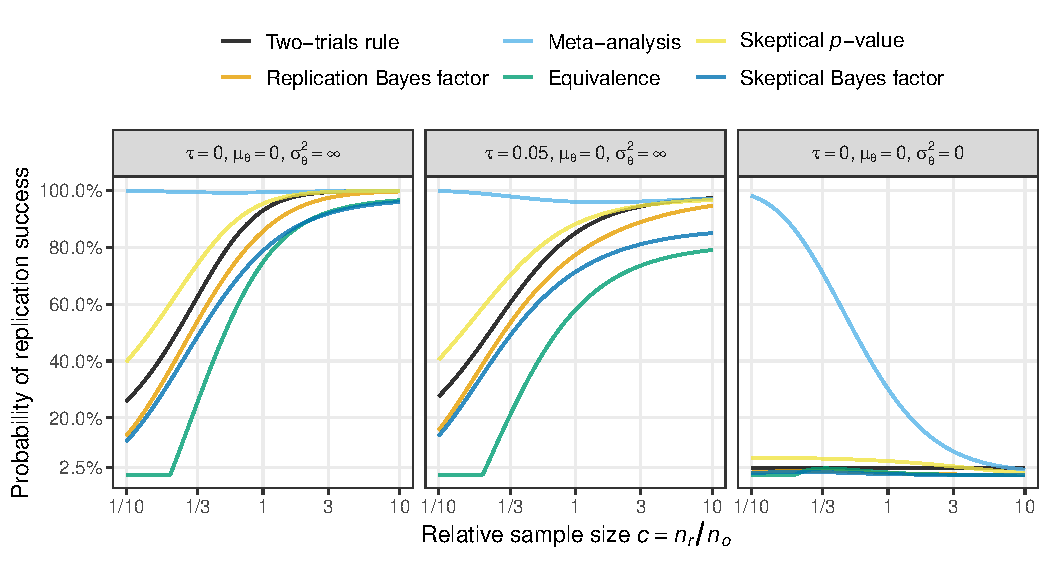
\includegraphics[width=\textwidth]{images/paper3/example-applied-1}
\end{knitrout}
\caption{Probability of replication success as a function of relative sample
  size $c = n_{r}/n_{o}$ for experiment ``Labels'' with original effect estimate
  $\hat{\theta}_{o} = 0.205$ and standard error $\sigma_{o} = 0.051$ for
  different initial prior parameters ($\tau, \mutheta, \sigmatheta^{2}$). The
  probability of replication success with the design prior
  \mbox{$\tau = 0, \mutheta = 0$, and $\sigmatheta^{2} = 0$} (right plot)
  corresponds to the type I error rate under the fixed effects null hypothesis
  ($H_{0}\colon \theta = 0, \tau^{2} = 0$). Replication success is defined by
  the two-trials rule at level $\alpha = 0.025$, the replication Bayes factor at
  level $\gamma = 1/10$, fixed effects-meta analysis at level
  $\alpha = 0.025^{2}$, effect size equivalence based on $90\%$ confidence
  interval and with margin $\Delta = 0.2$, sceptical $p$-value at level
  $\alpha = 0.062$, and sceptical Bayes factor at level $\gamma = 1/10$.}
\label{fig3:example}
\end{figure}
Figure~\ref{fig3:example} shows the probability of replication success as a
function of the relative sample size $c = n_{r}/n_{o}$ and for different initial
priors. The left and middle plot are based on an uninformative prior for the
effect size ($\sigmatheta^{2} \to \infty$) without heterogeneity ($\tau^{2} = 0$)
and with heterogeneity ($\tau^{2} = 0.05^{2}$),
respectively. The right plot shows the prior corresponding to the ``fixed
effects null hypothesis'' $H_{0} \colon \theta = 0, \tau^{2} =
0$, %, \ie{} the effect size
% $\theta$ is a point mass at zero and there is no heterogeneity,
so that the probability of replication success is the type I error rate which
some stakeholders might require to be ``controlled'' at some adequate level.

We see from the left and middle plots that increasing the relative sample size
monotonically increases the probability of replication success for all methods
but meta-analysis (light blue). Meta-analysis shows a non-monotone behavior
because the original study was already highly significant so that the pooled
effect estimate is significant even for replication studies with very small
sample size \citep{Micheloud2020}. The uncertainty regarding the replication
effect estimate $\that_{r}$ may therefore even reduce the probability of
replication success for meta-analysis if the sample size is increased. If
heterogeneity is taken into account (middle plot) the probability of replication
success becomes closer to 50\% for all methods but the equivalence test,
reflecting the larger uncertainty about the effect size $\theta$. To achieve
$80\%$ probability of replication success the fewest
samples are required with meta-analysis, followed by the sceptical $p$-value,
the two-trials rule, the replication Bayes factor, the sceptical Bayes factor,
and lastly the equivalence test. If the chosen sample size should guarantee a
sufficiently conclusive replication study with all these methods, the
replication sample size has to be slightly larger than the original one in the
situation of no heterogeneity ($\tau^{2} = 0$), while it has to be increased
more than ten-fold if there is heterogeneity
($\tau^{2} = 0.05^{2}$). However, this is mostly due to the
equivalence test which requires by far the most samples. If the equivalence test
sample size is ignored, the relative sample size
$c = 2.5$ ensures at least
$80\%$ probability of replication success with the
remaining methods.


The right plot in Figure~\ref{fig3:example} shows that the type I error rate of
the two-trials rule (black) stays constant at
$\alpha = 0.025$, as expected by definition of the method.
In contrast, the type I error rates of the other methods vary with the relative
sample size $c$ but most of them stay below
$\alpha = 0.025$ for all $c$ with the exception of
meta-analysis and the sceptical $p$-value. Meta-analysis (light blue) has an
extremely high type I error rate as the pooling with the highly significant
original data leads to replication success if the replication sample size is not
drastically increased. The type I error rate of the sceptical $p$-value (yellow)
is only slightly larger than $\alpha = 0.025$ which is
expected since the level $\alpha = 0.062$ is used for
declaring replication success with the sceptical $p$-value, and its type I error
rate is always smaller than the level for thresholding it \citep{Held2020}. The
type I error rate of the sceptical $p$-value decreases to values smaller than
$\alpha = 0.025$ of the two-trials rule at approximately
$c = 3$.





\begin{figure}[!htb]
\begin{knitrout}
\definecolor{shadecolor}{rgb}{0.969, 0.969, 0.969}\color{fgcolor}
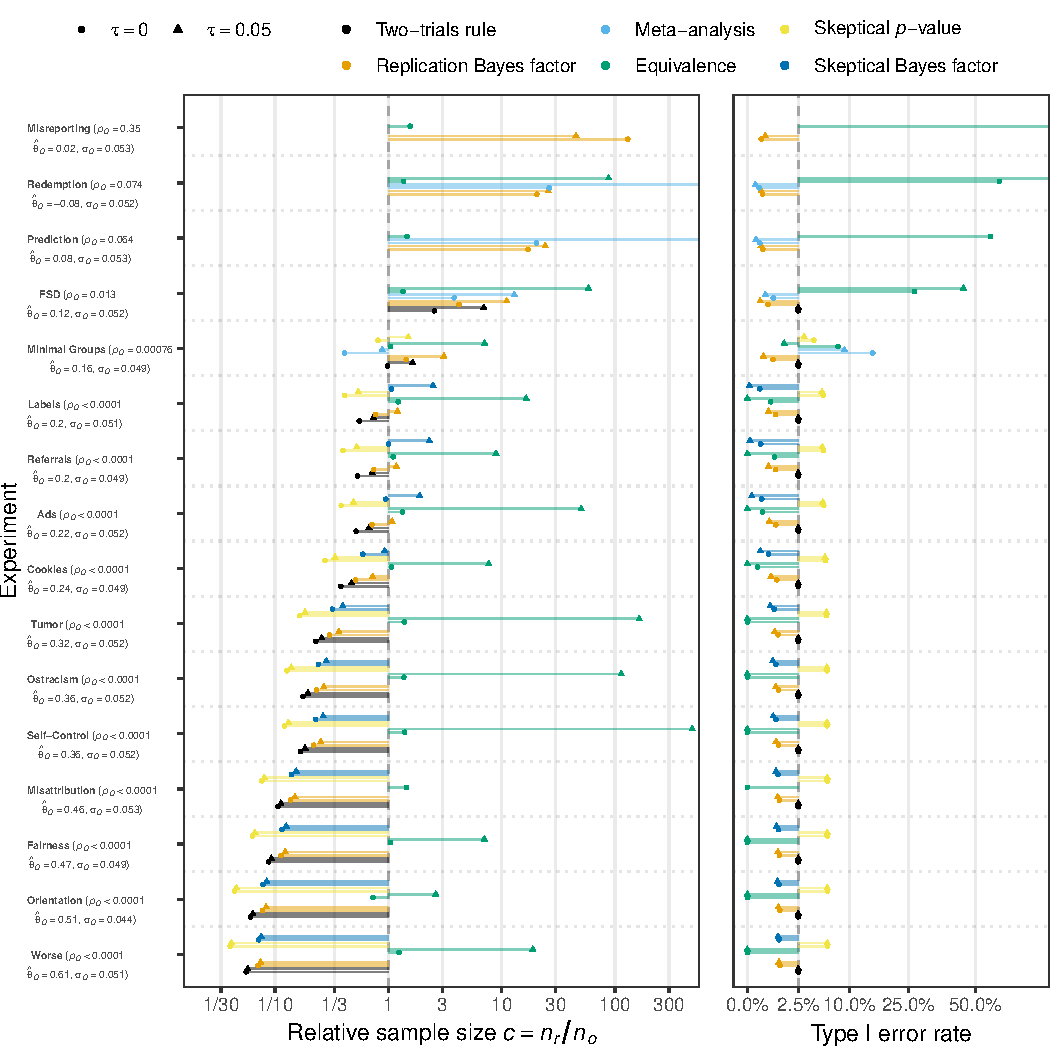
\includegraphics[width=\textwidth]{images/paper3/ssd-protzko-1}
\end{knitrout}
\caption{The left plot shows the required relative sample size $c = n_r/n_o$ to
  achieve a target probability of replication success of
  $1 - \beta = 80$\% (if possible). Replication success
  is defined through the two-trials rule at level $\alpha = 0.025$,
  replication Bayes factor at level $\gamma = 1/10$, fixed
  effects-meta analysis at level $\alpha = 0.025^{2}$,
  effect size equivalence at level $\alpha = 0.1$ with margin
  $\Delta = 0.2$, sceptical $p$-value at level
  $\alpha = 0.062$, and sceptical Bayes factor at level
  $\gamma = 1/10$ for data from the replication project by
  \citet{Protzko2020}. A flat initial prior
  ($\mutheta = 0, \sigmatheta^{2} \to \infty$) is used for the effect size
  $\theta$ is used either without ($\tau = 0$) or with heterogeneity
  ($\tau = 0.05$). The right plot shows the type I error
  rate associated with the required sample size. Experiments are ordered (top to
  bottom) by their original one-sided $p$-value
  $p_{o} = 1 - \Phi(|\hat{\theta}_{o}|/\sigma_{o}$).}
\label{fig3:ssd-all}
\end{figure}

We now conduct SSD for all studies from the replication project of
\citet{Protzko2020}. Figure~\ref{fig3:ssd-all} shows the required relative sample
size and the associated type I error rates if a sample size can be computed for
a probability of replication success of
$1 - \beta = 80$\%. If there is no sample size for
which a probability of $80$\% can be achieved the space
is left blank. This is, for instance, the case for the meta-analysis method for
all studies below the ``Labels'' experiment as the probability stays above
$80$\% for any relative sample size. % for the
% studies which were significant at level $\alpha = levelSig$ (so that
% they can fulfill the two-trials rule).

We see that for all methods but the equivalence test the required relative
sample size $c$ decreases with decreasing original $p$-value $p_{o}$, and
original studies with very small $p$-values require much fewer samples in the
replication study. For the equivalence test, the required sample size depends
instead on the size of the original standard error $\sigma_{o}$, and smaller
standard errors leads to smaller required sample sizes in the
replication. % For instance, the
% experiment ``Orientation'' with the original standard error $\sigma_{o} = 0.045$
% requires much less samples than the experiment ``Self-Control'' with original
% standard error $\sigma_{o} = 0.052$.
We also see that taking into account heterogeneity (triangle) increases the
required sample size for all methods compared to not taking it into account
(dot). At the same time, a larger required sample size reduces the type I error
rate for most methods. We see again the pattern that the type I error rate of
the equivalence test and the sceptical $p$-value is larger than the type I error
rate 2.5\% of the two-trials rule. However, while the type I error rate of the
sceptical $p$-value decreases when replication studies require larger sample
sizes, the type I error rate of the equivalence test may also be large if the
replication requires very large sample sizes (\eg{} for the experiment ``FSD'')
since it depends on whether the original effect estimate $\that_{o}$ is
sufficiently different from zero. If the original effect estimate $\that_{o}$ is
close to zero, the type I error rate of the equivalence test is drastically
increased as equivalence can also be established if the effect estimates from
original and replication studies are close to zero (as under the null
hypothesis).

Taken together, for most of the experiments all methods but the equivalence test
require fewer samples in the replication than in the original study to achieve a
target probability of replication success
$1 - \beta = 80$\%. This is still the case if
heterogeneity is taken into account in the design prior (triangles), which
generally increases the required sample size compared to when heterogeneity is
not taken into account (dots), especially for studies with large original
$p$-value. Larger replication sample sizes are required for some original
studies. In some cases these are unrealistically large (\eg{} in the experiment
``Prediction'' an almost 30 times increase in sample size for the replication
Bayes factor), but in other cases they seem more realistic and could be
reallocated from the other studies which require fewer samples (\eg{} in the
experiment ``Referrals'' an almost three times increase for the sceptical Bayes
factor). On the other hand, the equivalence test typically requires larger
sample sizes in the replication because the original standard errors are large
relative to the specified margin. If one anticipates to analyze the original and
replication pair with an equivalence test, this should therefore be taken into
account already at the design stage of the original study.

\subsection{Sample size determination for multisite replication projects}
So far we considered the situation where a pair of a single original and a
single replication study are analyzed in isolation. However, if multiple
replications per single original study are conducted (so-called \emph{multisite}
replication studies) the ensemble of replications can also be analyzed jointly.
In this case, some adaptations of the SSD methodology are required.

The replication effect estimate and its standard error are now vectors
$\bthat_{r} = (\that_{r1}, \dots, \that_{rm})^{\top}$ and
$\bsigma^{2}_{r} = (\sigma^{2}_{r1}, \dots, \sigma^{2}_{rm})^{\top}$ consisting
of $m$ replication effect estimates, respectively, their standard errors. The
normal hierarchical model for the replication estimates $\bthat_{r}$ then
becomes
\begin{subequations}
\label{eq3:hierarch-model2}
\begin{align}
  \bthat_r \given \mspace{-1mu} \btheta_r &\sim \Nor_{m}\left\{\btheta_r, \mathrm{diag}\left(\bsigma_r^2\right)\right\}
  \label{eq3:hat_theta_k22} \\
  \btheta_r \given \theta \,\,  &\sim \Nor_{m}\left\{\theta \, \bone_{m},
  \tau^2 \mathrm{diag}(\bone_{m})\right\}, \label{eq3:theta_k2}
\end{align}
\end{subequations}
where $\btheta_{r}$ is a vector of $m$ study specific effect sizes, $\bone_{m}$
is a vector of $m$ ones, and $\Nor_{m}(\boldsymbol{\mu}, \boldsymbol{\Sigma})$
denotes the $m$-variate normal distribution with mean vector $\boldsymbol{\mu}$
and covariance matrix $\boldsymbol{\Sigma}$. By marginalizing over the study
specific effect size $\btheta_{k}$, the model can alternatively be expressed by
\begin{align}
  \bthat_r \given \theta \sim \Nor_{m}\left\{\theta \, \bone_{m},
\mathrm{diag}\left(\bsigma_r^2 + \tau^2 \bone_{m}\right)\right\},
  \label{eq3:margimulti}
\end{align}
so the predictive distribution of $\bthat_r$ based on the design
prior~\eqref{eq3:dpnormal} is given by
\begin{align}
  \bthat_r \given \hat{\theta}_o, \sigma^{2}_{o}, \bsigma^{2}_{r}
  \sim \Nor_{m}\left\{\muthatr \bone_{m},
  \mathrm{diag}\left(\bsigma_r^2 + \tau^2 \bone_{m}\right) +
  \left(\frac{\tau^{2} + \sigma^{2}_{o}}{1 + 1/g}\right)
  \bone_{m} \bone_{m}^{\top} \right\}
  \label{eq3:ftrmulti}
\end{align}
with $ \muthatr$ the mean of the predictive distribution of a single replication
effect estimate from~\eqref{eq3:fthetar}. Importantly, the replication effect
estimates are correlated as the covariance matrix in~\eqref{eq3:ftrmulti} has
$(\tau^2+\sigma^{2}_{o})/(1 + 1/g)$ in the off-diagonal entries.

Often the assessment of replication success can be formulated in terms of a
weighted average of the replication effect estimates
$\hat{\theta}_{r*} = (\sum_{i = 1}^{m} w_{i} \hat{\theta}_{ri})/(\sum_{i = 1}^{m} w_{i})$
with $w_{i}$ the weight of replication $i$. For instance, several multisite
replication projects \citep[\eg][]{Klein2018} have defined replication success
by the fixed or random effects meta-analytic effect estimate of the replication
effect estimates achieving statistical significance. Based on the predictive
distribution of the replication effect estimate vector~\eqref{eq3:ftrmulti}, the
predictive distribution of the weighted average $\hat{\theta}_{r*}$ is given by
\begin{align}
  \hat{\theta}_{r*} \given \hat{\theta}_o, \sigma^{2}_{o}, \bsigma^{2}_{r}
  \sim \Nor\Biggl\{
  \mu_{\scriptscriptstyle \that_{r}},
  \sigma^{2}_{\scriptscriptstyle \that_{r*}} =
  \biggl(\sum_{i=1}^{m} w_{i}^{2} \sigma^{2}_{\scriptscriptstyle \that_{ri}} +
  \sum_{i=1}^{m}\sum_{\substack{j =1 \\ j\neq i}}^{m} w_{i}w_{j}
\frac{\tau^{2} + \sigma^{2}_{o}}{1 + 1/g} \biggr)\big/\biggl(\sum_{i=1}^{m} w_{i}\biggr)^{2} \Biggr\}
  \label{eq3:ftwm}
\end{align}
with $\sigma^{2}_{\scriptscriptstyle \that_{ri}}$ the predictive variance of a
single replication effect estimate with standard error $\sigma_{ri}$ as
in~\eqref{eq3:fthetar}. In particular when the studies receive equal weights
($w_{i} = w$ for $i = 1, \dots, m$) and the standard errors of the replication
effect estimates are equal ($\sigma_{ri} = \sigma_{r}$ for $i = 1, \dots, m$),
the predictive variance becomes
\begin{align}
  \sigma^{2}_{\scriptscriptstyle \that_{r*}} =
  % \left(\sigma^{2}_{\scriptscriptstyle \that_{r}} + (n - 1) \frac{g}{g + 1} [\tau^{2} + \sigma^{2}_{o}]\right) \big/ n.
  \frac{\sigma^{2}_{r} + \tau^{2}}{m} + \frac{\tau^{2} + \sigma^{2}_{o}}{1 + 1/g}.
  \label{eq3:predvarequal}
\end{align}
The probability of replication success can now be obtained by
integrating~\eqref{eq3:ftrmulti}, respectively~\eqref{eq3:ftwm}, over the
corresponding success region $S$. This may be more involved if the success
region is defined in terms of the replication effect estimate vector
$\bthat_{r}$, whereas it is as simple as in the singlesite replication case if
the success region is formulated in terms of the weighted average $\that_{r*}$.


\subsubsection{Optimal allocation within and between sites}
A key challenge in SSD for multisite replication studies is the optimal
allocation of samples within and between sites, that is, how many sites $m$ and
how many samples $n_{ri}$ per site $i$ should be used. A similar problem exists
in SSD for cluster randomized trials and we can adapt the common solution based
on cost functions \citep{Raudenbush1997}. %\citep[chapter 9.6]{Cochran1977}.
That is, the optimal configuration is determined so that the probability of
replication success is maximized subject to a constrained cost function which
accounts for the (typically different) costs of additional samples and sites.

For example, assume a balanced design ($n_{ri} = n_{r}$ for $i = 1, \dots, m$)
and that the standard errors of the replication effect estimates are inversely
proportional to the square-root of the sample size
$\sigma_{ri} = \lambda/\sqrt{n_{r}}$ for some unit variance $\lambda^{2}$.
Further assume that maximizing the probability of replication success
corresponds to minimizing the variance of the weighted average
$\sigma^{2}_{\scriptscriptstyle \that_{r*}}$ in~\eqref{eq3:predvarequal}. % This
% is, for instance, the case if the analysis consists of computing a $p$-value for
% the weighted average.
Let $K_{s}$ denote the cost of an additional site, and $K_{c}$ the cost of an
additional sample/case. The total cost of the project is then
$K = m(K_{c} \, n_{r} + K_{s})$, and constrained minimization of the predictive
variance~\eqref{eq3:predvarequal} leads to the optimal sample size per site
\begin{align*}
  n_{r}^{*} =  \frac{\lambda}{\tau} \, \sqrt{\frac{K_{s}}{K_{c}}}
\end{align*}
which is equivalent to the optimal cluster sample size known from cluster
randomized trials \citep{Raudenbush2000}. Note that the optimal sample size per
site may be different for other analysis approaches where maximizing the
probability of replication success does not correspond to minimizing the
variance of the weighted average. % \citep[for optimal
% % sample sizes for estimation of between replication variances see
% % \eg][]{Hedges2021}.
% % For example, \citet{Hedges2021}
% % found that the optimal sample size for between study variance estimation is
% % given by
% % \begin{align*}
% %   n_{r}^{*} =  \frac{1 + \sqrt{1 + 8\tau^{2} K_{s}/K_{i}}}{2 \tau^{2}/\lambda^{2}}.
% % \end{align*}
Moreover, there are also practical considerations which affect the choice of how
many sites should be included in a project. For instance, there may simply not
be enough labs available with the required expertise to perform the replication
experiments.

\subsection{Example: Cross-laboratory replication project (continued)}
Figure~\ref{fig3:multisite} illustrates multisite SSD for the experiment
``Labels'' from \citet{Protzko2020} for planned analyses based on the
two-trials rule and the replication Bayes factor (see the supplement for details
on the multisite extension of these two methods). As for singlesite SSD, we use
the design prior based on an initial flat prior for the effect size and taking
into account heterogeneity ($\tau = 0.05$). The top
plots show the probability of replication success as a function of the total
sample size $m \times n_{r}$ for different number of sites $m$. We see that for
the same total sample size a larger number of sites increases the probability of
replication success. For instance, a total sample size of roughly 3000 is
required to achieve an 80\% target probability with one site %(yellow)
for the two-trials rule, whereas only approximately half as many samples are
required for two sites. %(green).


\begin{figure}[!htb]
\begin{knitrout}
\definecolor{shadecolor}{rgb}{0.969, 0.969, 0.969}\color{fgcolor}
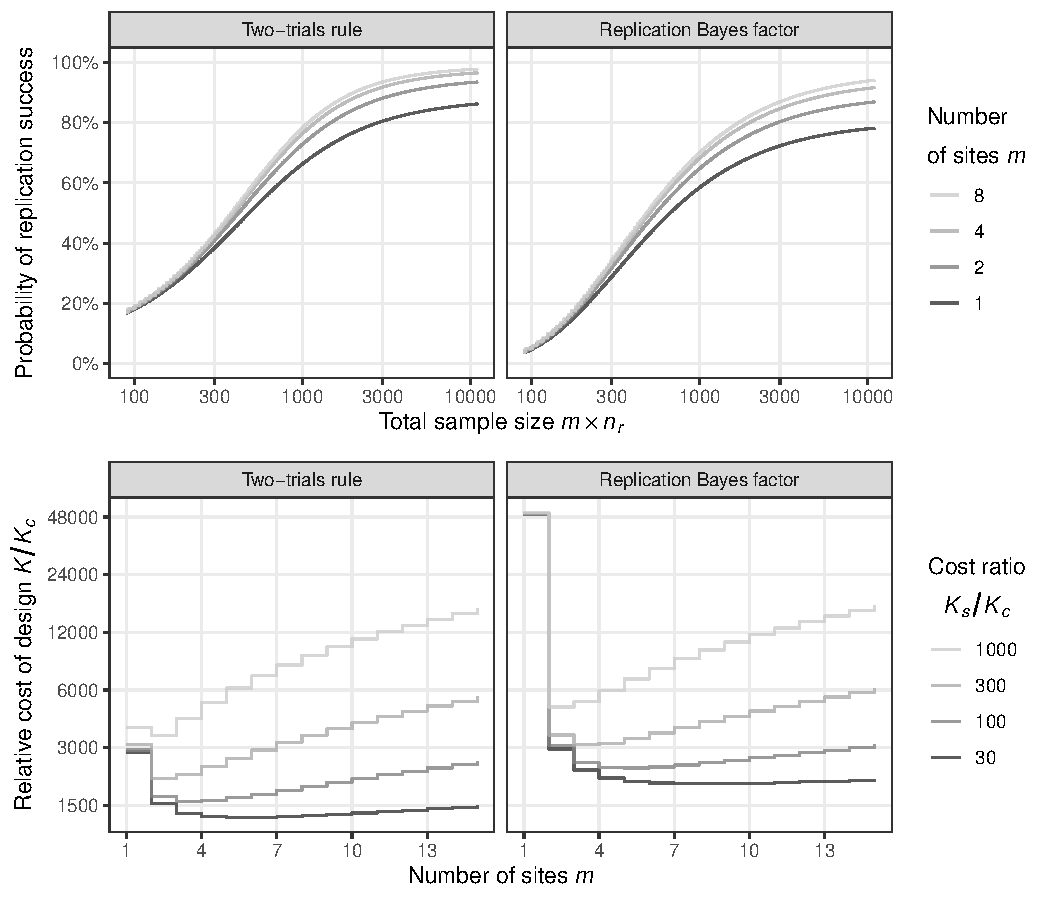
\includegraphics[width=\textwidth]{images/paper3/multisite-protzko-1}
\end{knitrout}
\caption{Top plots show the probability of replication success based on the
  replication Bayes factor at level $\gamma = 1/10$ (left) and the
  two-trials rule at level $\alpha = 0.025$ (right) as a function of
  the total sample size and for different number of sites $m$ for data from the
  experiment ``Labels''. A design prior with heterogeneity
  $\tau = 0.05$ and flat initial prior for the effect size
  $\theta$ is used. The same heterogeneity value is assumed in the analysis of the
  replications. %($\tau_{r} = \tau$). Bottom plot shows the total cost $K$ of the
  design (relative to the cost of a single sample $K_{c}$) as a function of the
  number of sites $m$ and for different site costs $K_{s}$. The sample size of
  each design corresponds to a target probability of replication success
  $1 - \beta = 80$\%.}
\label{fig3:multisite}
\end{figure}

However, focusing only on the total sample size ignores the fact that the cost
of an additional site is usually larger than the cost of an additional
observation. The bottom plot shows the total cost $K$ of a design (relative to
the cost of one sample $K_{c}$) whose sample size is determined for a target
probability of replication success $1 - \beta = 80$\%.
We see that if the cost of an additional site $K_{s}$ is not much larger than
the cost of an additional sample $K_{c}$, \eg{} $K_{S}/K_{c} = 30$ %(yellow)
the optimal number of sites is $m = 5$ for the two-trials rule and $m = 8$ for
the replication Bayes factor. If an additional site is more costly the optimal
number of sites is lower, \eg{} if the cost ratio is $K_{S}/K_{c} = 300$,
% (purple),
the optimal number of sites is $m = 2$ for the two trials rule and $m = 3$ for
the replication Bayes factor. This is similar to the actually used number of
sites $m = 3$ (counting only external-replications), respectively, $m = 4$
(counting also the internal-replication) from \citet{Protzko2020}.

\section{Discussion}
\label{sec3:discussion}

We showed how Bayesian approaches can be used to determine the sample size of
replication studies based on all the available information and the associated
uncertainty. % The Bayesian framework allows to make use of all the available
% information, and to take into account the associated uncertainty.
A key strength of the approach is that it can be applied to any kind of
replication analysis method, Bayes or non-Bayes, as long as there is a
well-defined success region for the replication effect estimate. Methods for
assessing replication success which have not yet been adapted to Bayesian design
approaches in the normal-normal hierarchical model (or which have not even been
proposed) can thus benefit from our methodology. For instance, our methods could
be straightforwardly applied to the ``dual-criterion'' from
\citet{Rosenkranz2021} which defines replication success via simultaneous
statistical significance and practical relevance of the effect estimates from
original and replication study.

There are some limitations and possible extensions: we have developed the
methodology for ``direct'' replication studies \citep{Simons2014} which attempt
to replicate the conditions from the original study as closely as possible; yet
SSD methodology is also needed for ``conceptual'' replication and for
``generalization'' studies which may show systematic deviations from the
original study. While the heterogeneity variance in the design prior allows to
take effect size heterogeneity into account for SSD, to some extent, further
research is needed for investigating how systematic study deviations and
external knowledge can be incorporated. Furthermore, as is standard in
meta-analysis we assumed that the variances of the effect estimates are known,
which can sometimes be inadequate \citep{Jackson2018}. Specifying priors also
for the variances could better reflect the available uncertainty but would come
at the price of lower interpretability and higher computational complexity. We
did also not consider designs where the replication data are analyzed in a
sequential manner. Ideas from the Bayesian sequential design
\citep{Schoenbrodt2017, Stefan2022} or from the adaptive trials literature
\citep{Bretz2009} could be adapted to the replication setting as in
\citet{Micheloud2020}. A sequential analysis of the replication data could
possibly increase the efficiency of the replication. An additional point is that
we assumed that the original study has been completed when planning the
replication study. One could also consider a scenario where both the original
and replication study are planned simultaneously and adopt a ``project''
perspective \citep{Maca2002, Held2021}. However, in this case no information from
the original study is available and the design prior needs to be specified
entirely based on external knowledge. Finally, researchers have only limited
resources and it may happen that they cannot afford a large enough sample size
to obtain their desired probability of replication success. In this situation a
reverse-Bayes approach \citep{Held2021b} could be applied in order to determine
the prior for the effect size which is required to achieve the desired
probability of replication success based on the maximally possible sample size.
Researchers can then judge whether or not such prior beliefs are scientifically
sensible, and decide whether they should conduct the replication study with
their limited resources.

\section*{Software and data}
All our analyses were conducted in the R programming language version 4.2.2
\citep{R}. Code to reproduce this manuscript is available at
\url{https://github.com/SamCH93/BAtDRS}. A snapshot of the Git repository at the
time of writing is archived at \url{https://doi.org/10.5281/zenodo.7291076}.
Methods for Bayesian design of replication studies are implemented in the R
package BayesRepDesign which is available at
\url{https://github.com/SamCH93/BayesRepDesign}. The CC-By 4.0 licensed data
were downloaded from \url{https://osf.io/42ef9/}. The R markdown script
``Decline effects main analysis.Rmd'' was executed and the relevant variables
from the objects ``ES\_experiments'' and ``decline\_effects'' were saved.

\section*{Acknowledgments}
% This work was supported by the Swiss National Science Foundation (\#189295). The
% funder had no role in study design, data collection, data analysis, data
% interpretation, decision to publish, or preparation of the manuscript.
We thank \citet{Protzko2020} for publicly sharing their data. We thank Charlotte
Micheloud and Angelika Stefan for helpful comments on drafts of the manuscript.
Our acknowledgment of these individuals does not imply their endorsement of this
article.

\begin{subappendices}
\renewcommand{\thesection}{\Alph{section}}
\section{The BayesRepDesign R package}
\label{app3:package}

\begin{knitrout}\footnotesize
\definecolor{shadecolor}{rgb}{0.969, 0.969, 0.969}\color{fgcolor}\begin{kframe}
\begin{alltt}
\hlkwd{library}\hlstd{(}\hlstr{"BayesRepDesign"}\hlstd{)}

\hlcom{## design prior (flat initial prior for effect size + heterogeneity)}
\hlstd{dp} \hlkwb{<-} \hlkwd{designPrior}\hlstd{(}\hlkwc{to} \hlstd{=} \hlnum{0.2}\hlstd{,} \hlkwc{so} \hlstd{=} \hlnum{0.05}\hlstd{,} \hlkwc{tau} \hlstd{=} \hlnum{0.08}\hlstd{)}
\hlkwd{plot}\hlstd{(dp)}
\end{alltt}
\end{kframe}
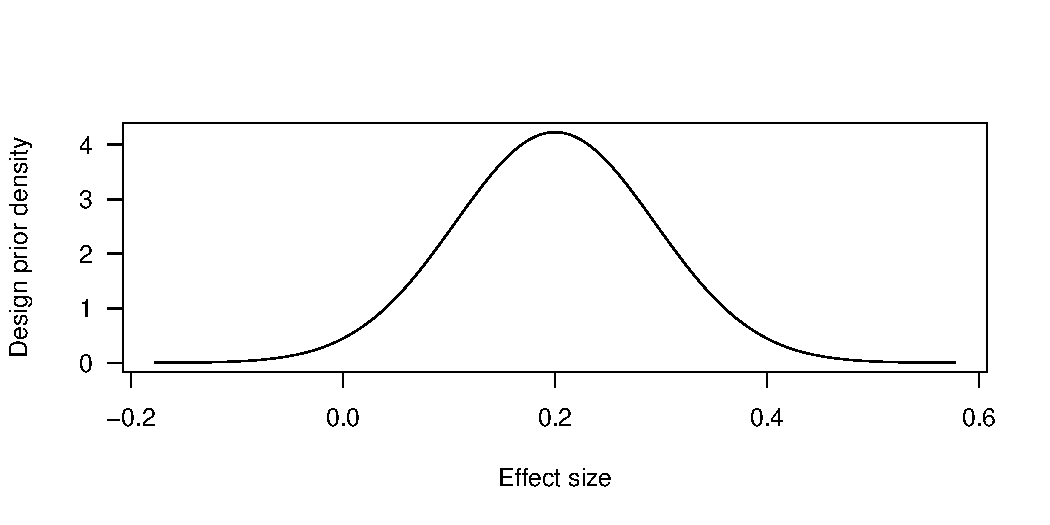
\includegraphics[width=0.9\textwidth]{images/paper3/package-illustration-1}
\begin{kframe}\begin{alltt}
\hlcom{## compute replication standard error for achieving significance at 2.5%}
\hlkwd{ssdSig}\hlstd{(}\hlkwc{level} \hlstd{=} \hlnum{0.025}\hlstd{,} \hlkwc{dprior} \hlstd{= dp,} \hlkwc{power} \hlstd{=} \hlnum{0.8}\hlstd{)}
\end{alltt}
\begin{verbatim}
##        Bayesian sample size calculation for replication studies
##        ========================================================
##
## success criterion and computation
## ------------------------------------------------------------------------
##   replication p-value <= 0.025 (exact computation)
##
## original data and initial prior for effect size
## ------------------------------------------------------------------------
##   to = 0.2 : original effect estimate
##   so = 0.05 : standard error of original effect estimate
##   tau = 0.08 : assumed heterogeneity standard deviation
##   N(mean = 0, sd = Inf) : initial normal prior
##
## design prior for effect size
## ------------------------------------------------------------------------
##   N(mean = 0.2, sd = 0.094) : normal design prior
##
## probability of replication success
## ------------------------------------------------------------------------
##   PoRS = 0.8 : specified
##   PoRS = 0.8 : recomputed with sr
##
## required sample size
## ------------------------------------------------------------------------
##   sr = 0.045 : required standard error of replication effect estimate
##   c = so^2/sr^2 ~= nr/no = 1.2 : required relative variance / sample size
\end{verbatim}
\begin{alltt}
\hlcom{## compute numerically via success region and method agnostic function}
\hlstd{sregFun} \hlkwb{<-} \hlkwa{function}\hlstd{(}\hlkwc{sr}\hlstd{) \{}
    \hlcom{## success region is [1.96*sr, Inf)}
    \hlkwd{successRegion}\hlstd{(}\hlkwc{intervals} \hlstd{=} \hlkwd{cbind}\hlstd{(}\hlkwd{qnorm}\hlstd{(}\hlkwc{p} \hlstd{=} \hlnum{0.975}\hlstd{)}\hlopt{*}\hlstd{sr,} \hlnum{Inf}\hlstd{))}
\hlstd{\}}
\hlkwd{ssd}\hlstd{(}\hlkwc{sregionfun} \hlstd{= sregFun,} \hlkwc{dprior} \hlstd{= dp,} \hlkwc{power} \hlstd{=} \hlnum{0.8}\hlstd{)}
\end{alltt}
\begin{verbatim}
##        Bayesian sample size calculation for replication studies
##        ========================================================
##
## success criterion and computation
## ------------------------------------------------------------------------
##   method agnostic success region (numerical computation)
##
## original data and initial prior for effect size
## ------------------------------------------------------------------------
##   to = 0.2 : original effect estimate
##   so = 0.05 : standard error of original effect estimate
##   tau = 0.08 : assumed heterogeneity standard deviation
##   N(mean = 0, sd = Inf) : initial normal prior
##
## design prior for effect size
## ------------------------------------------------------------------------
##   N(mean = 0.2, sd = 0.094) : normal design prior
##
## probability of replication success
## ------------------------------------------------------------------------
##   PoRS = 0.8 : specified
##   PoRS = 0.8 : recomputed with sr
##
## required sample size
## ------------------------------------------------------------------------
##   sr = 0.045 : required standard error of replication effect estimate
##   c = so^2/sr^2 ~= nr/no = 1.2 : required relative variance / sample size
\end{verbatim}
\end{kframe}
\end{knitrout}

\section{Supplementary material}

Here, we provide additional information on computing the predictive distribution
of the replication effect estimate when a prior is assigned to the heterogeneity
variance $\tau^{2}$ (Section~\ref{sec3sup:priortau}). We also provide additional
information on methods for analyzing replication data. For each method we derive
the \emph{success region} in terms of the effect estimate of the replication
study $\that_{r}$, which is required for sample size determination as
illustrated in the main manuscript (Section~\ref{sec3sup:2TR} to~\ref{sec3sup:BFs}). For
the two-trials rule and the replication Bayes factor methods we additionally
provide derivations on how these methods can be generalized to the multisite
replication setting. We show then how the optimal number of samples per site can
be derived for multisite SSD (Section~\ref{sec3sup:multi}). Finally, we show SSD for
the \citet{Protzko2020} project but using an adaptive shrinkage prior instead of
the flat prior as in the main manuscript (Section~\ref{sec3sup:ssdprotzko}).

\subsection{Prior on the heterogeneity variance}
\label{sec3sup:priortau}
When also a prior is assigned to the heterogeneity variance $\tau^{2}$, the
predictive distribution of the replication effect estimate $\that_{r}$ is given
by
\begin{align*}
  f(\that_{r} \given \that_{o}, \sigma_{o}, \sigma_{r})
  &= \int_{0}^{+\infty} f(\that_{r} \given \sigma_{r}, \that_{o}, \sigma_{o},
    \tau^{2}) \,
    f(\tau^{2} \given \that_{o}, \sigma_{o}) \, \mathrm{d}\tau^{2}.
\end{align*}
That is, it is the predictive distribution of the replication effect estimate
$\that_{r}$ integrated with respect to the marginal posterior of $\tau^{2}$
based on the original data $x_{o} = \{\that_{o}, \sigma^{2}_{o}\}$. If the
initial prior for $\theta$ is normal
$\theta \sim \Nor(\mutheta, \sigmatheta^{2})$, and the initial prior for
$\tau^{2}$ has density $f(\tau^{2})$, we have
\begin{align*}
  f(\tau^{2} \given \that_{o}, \sigma_{o})
  &= \int_{-\infty}^{+\infty} f(\theta, \tau^{2} \given \that_{o}, \sigma_{o}) \, \mathrm{d}\theta \\
  &= \frac{\int_{-\infty}^{+\infty} f(\that_{o} \given \theta, \tau^{2}, \sigma^{2}_{o}) \,
    f(\theta \given \tau^{2}) \, f(\tau^{2}) \, \mathrm{d}\theta}{\int_{0}^{+\infty}
    \int_{-\infty}^{+\infty} f(\that_{o} \given \theta_{*}, \tau^{2}_{*}, \sigma^{2}_{o}) \,
    f(\theta_{*} \given \tau^{2}_{*}) \, f(\tau^{2}_{*}) \, \mathrm{d}\theta_{*} \,
    \mathrm{d}\tau^{2}_{*}} \\
  &= \frac{f(\tau^{2}) \int_{-\infty}^{+\infty} \Nor(\that_{o} \given \theta, \tau^{2}
    + \sigma^{2}_{o}) \, \Nor(\theta \given \mutheta, \sigmatheta^{2}) \,\mathrm{d}\theta
    }{\int_{0}^{+\infty} f(\tau^{2}_{*})
    \int_{-\infty}^{+\infty} \Nor(\that_{o} \given \theta_{*}, \tau^{2}_{*} + \sigma^{2}_{o}) \,
    \Nor(\theta_{*} \given \mutheta, \sigmatheta^{2}) \, \mathrm{d}\theta_{*} \,
    \mathrm{d}\tau^{2}_{*}} \\
  &= \frac{f(\tau^{2}) \, \Nor(\that_{o} \given \mutheta, \tau^{2}
    + \sigma^{2}_{o} + \sigmatheta^{2})
    }{\int_{0}^{+\infty} f(\tau^{2}_{*})
    \Nor(\that_{o} \given \mutheta, \tau^{2}_{*} + \sigma^{2}_{o} + \sigmatheta^{2}) \,
    \mathrm{d}\tau^{2}_{*}}.
\end{align*}
To compute the marginal posterior density of $\tau^{2}$ one numerical
integration is hence required. The updating of the prior depends on the distance
between prior mean $\mutheta$ and the original effect estimate $\that_{o}$
relative to the prior variance $\sigmatheta^{2}$ and the squared standard error
$\sigma_{o}^{2}$. If an improper uniform prior is assigned to $\theta$
($\sigmatheta^{2} \to \infty$), the posterior reduces to the prior
\begin{align*}
  \lim_{\sigmatheta^{2} \to \infty} f(\tau^{2} \given \that_{o}, \sigma_{o})
  &= \lim_{\sigmatheta^{2} \to \infty} \frac{f(\tau^{2}) \, \Nor(\that_{o} \given \mutheta, \tau^{2}
    + \sigma^{2}_{o} + \sigmatheta^{2})
    }{\int_{0}^{+\infty} f(\tau^{2}_{*})
    \Nor(\that_{o} \given \mutheta, \tau^{2}_{*} + \sigma^{2}_{o} + \sigmatheta^{2}) \,
    \mathrm{d}\tau^{2}_{*}} \\
  &= \lim_{\sigmatheta^{2} \to \infty}  \int_{0}^{+\infty} \frac{f(\tau^{2})}{f(\tau^{2}_{*})} \,
    \underbrace{\sqrt{\frac{\tau^{2}_{*} + \sigma^{2}_{o} + \sigmatheta^{2}}{\tau^{2} + \sigma^{2}_{o} +
    \sigmatheta^{2}}}}_{\to 1} \\
  &\phantom{= \lim_{\sigmatheta^{2} \to \infty}  \int_{0}^{+\infty}} \times \exp\bigg[-\frac{1}{2}\bigg\{\underbrace{
    \frac{(\that_{o} - \mutheta)^{2}}{\tau^{2} + \sigma^{2}_{o} + \sigmatheta^{2}}}_{\downarrow 0} -
    \underbrace{\frac{(\that_{o} - \mutheta)^{2}}{\tau^{2}_{*} + \sigma^{2}_{o} +
    \sigmatheta^{2}}}_{\downarrow 0} \bigg\}\bigg] \, \mathrm{d}\tau^{2}_{*} \\
  &= f(\tau^{2}),
\end{align*}
the limit can be interchanged with the integral because of the monotone
convergence theorem. This means that with a uniform prior nothing can be learned
about the variance $\tau^{2}$ which intuitively makes sense as estimation of a
variance requires at least two observations. The phenomenon is illustrated in
Figure~\ref{fig3sup:margposttau2} for the data from the experiment ``Labels''
\citep{Protzko2020} as also used in the main manuscript. We see that as the
prior standard deviation increases (making the prior more uniform), the marginal
posterior density becomes closer to the prior density.
\begin{figure}[!htb]
\begin{knitrout}
\definecolor{shadecolor}{rgb}{0.969, 0.969, 0.969}\color{fgcolor}
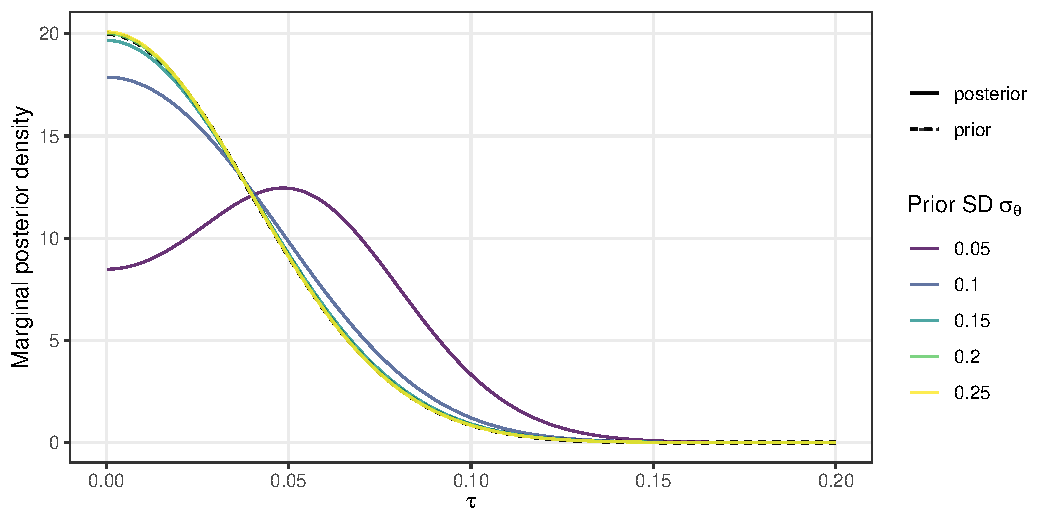
\includegraphics[width=\maxwidth]{images/paper3/sup-tau-random-example-1}
\end{knitrout}
\caption{Marginal posterior distribution of heterogeneity variance $\tau^{2}$
  based on data from experiment ``Labels'' from \citet{Protzko2020} with
  original effect estimate $\hat{\theta}_{o} = 0.205$ and
  standard error $\sigma_{o} = 0.051$. A
  $\theta \sim \Nor(0, \sigmatheta^{2})$ prior is assigned to the
  effect size $\theta$ and a half normal prior with standard deviation
  $0.04$ is assigned to $\tau$.}
\label{fig3sup:margposttau2}
\end{figure}

Combining all the previous results, we obtain the probability of replication
success as
\begin{align*}
  \Pr(\that_{r} \in S \given \that_{o}, \sigma_{o}, \sigma_{r})
  &= \int_{S}\int_{0}^{+\infty} f(\that_{r} \given \that_{o}, \sigma_{o}, \sigma_{r}, \tau^{2}) \,
    f(\tau^{2} \given \that_{o}, \sigma_{o}) \, \mathrm{d}\that_{r} \,\mathrm{d}\tau^{2} \\
  &= \int_{0}^{+\infty} \Pr(\that_{r} \in S \given \that_{o}, \sigma_{o}, \sigma_{r}, \tau^{2}) \,
    f(\tau^{2} \given \that_{o}, \sigma_{o}) \, \mathrm{d}\tau^{2}. \\
\end{align*}
This mean computing the probability of replication success with a prior on
$\tau^{2}$ requires two-dimensional numerical integration. However, in the
common case when a uniform prior is assigned to $\theta$, the marginal posterior
distribution of $\tau^{2}$ reduces to the prior, and only one numerical
integration is required.

\begin{figure}[!htb]
\begin{knitrout}
\definecolor{shadecolor}{rgb}{0.969, 0.969, 0.969}\color{fgcolor}
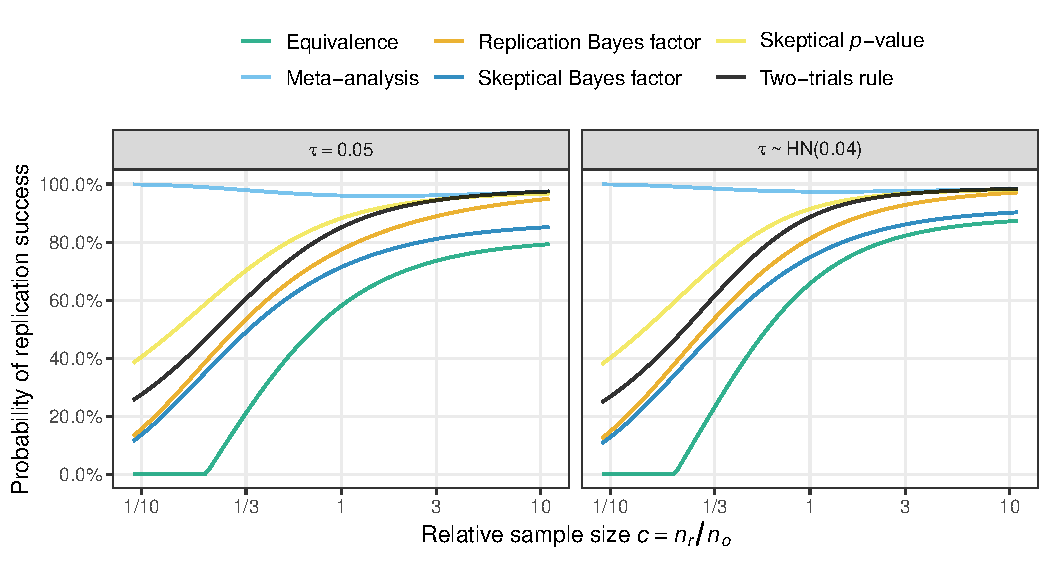
\includegraphics[width=\maxwidth]{images/paper3/sup-example-applied-1}
\end{knitrout}
\caption{Probability of replication success as a function of relative sample
  size $c = n_{r}/n_{o}$ for experiment ``Labels'' with original effect estimate
  $\hat{\theta}_{o} = 0.205$ and standard error $\sigma_{o} = 0.051$ for uniform
  initial prior for effect size $\theta$ and either fixed $\tau = 0.05$ (as in
  main manuscript) or half normal prior with standard deviation $0.04$ assigned
  to $\tau$. Replication success is defined by the two-trials rule at level
  $\alpha = 0.025$, the replication Bayes factor at level $\gamma = 1/10$, fixed
  effects-meta analysis at level \mbox{$\alpha = 0.025^{2}$}, effect size
  equivalence based on $90\%$ confidence interval and with margin
  $\Delta = 0.2$, sceptical $p$-value at level $\alpha = 0.062$, and sceptical
  Bayes factor at level $\gamma = 1/10$.}
\label{fig3sup:exampletaurandom}
\end{figure}

Figure~\ref{fig3sup:exampletaurandom} shows the probability of replication
success based on data from the ``Labels'' experiment, as in the main manuscript.
A half normal prior with is assigned to the heterogeneity $\tau$ which is a
typical prior distribution used for heterogeneity modeling in meta-analysis
\citep{Rover2021}. The standard deviation of the prior is set to $0.04$ so that
the mean of the prior equals the value of the fixed heterogeneity $\tau = 0.05$
elicited in the main manuscript. We see that the probability of replication
success is only slightly higher compared to the fixed $\tau = 0.05$ from the
main manuscript.


\subsection{The two-trials rule}
\label{sec3sup:2TR}
\sloppy
The two-trials rule is the most common analysis approach for replication
studies. Replication success is declared if both original and replication study
achieve statistical significance at some level $\alpha$ (and both estimates go
in the same direction which can be taken into account by using one-sided
$p$-values). We will study the two-trial under normality using the data model
$\that_{i} \given \theta \sim \Nor(\theta, \sigma^{2}_{i})$ with $\that_{i}$ the
estimate of the unknown effect size $\theta$ from study $i$ and $\sigma_{i}$ is
the corresponding standard error (assumed to be know). The $p$-values for
testing $H_{0} \colon \theta = 0$ versus $H_{1} \colon \theta > 0$ are then
$p_{i} = 1 - \Phi(\that_{i}/\sigma_{i})$ whereas for the alternative
$H_{1} \colon \theta < 0$ they are $p_{i} = \Phi(\that_{i}/\sigma_{i})$. Suppose
the original effect estimate was statistically significant at level $\alpha$,
\ie{} \mbox{$p_{o} \leq \alpha$}. Replication success at level $\alpha$ is then
established if the replication effect estimate $\that_{r}$ is also statistically
significant at level $\alpha$, \ie{} $p_{r} \leq \alpha$. By applying some
algebraic manipulations to the success condition, one can show that this implies
that replication success is achieved if the replication effect estimate
$\that_{r}$ is contained in the success region
\begin{align*}
  S_{\mathrm{2TR}} =
  \begin{cases}
    \left[\zalpha \, \sigma_{r}, \infty \right) & \mathrm{for} ~ \that_{o} > 0 \\
    \left[-\infty, -\zalpha \, \sigma_{r} \right) & \mathrm{for} ~ \that_{o} < 0.
  \end{cases}
\end{align*}

\subsubsection{The multisite two-trials rule}
If multiple replication studies are conducted for one original study (a
\emph{multisite} replication), the two-trials rule is typically modified by
meta-analyzing the effect estimates from all replications and then using the
combined estimate as usual in the two-trials rule \citep[see \eg{} the ``Many
labs'' projects from][]{Klein2014, Klein2018}. Suppose $m$ replication studies
are conducted and produce $m$ effect estimates $\that_{r1}, \dots, \that_{m}$
with standard errors $\sigma_{r1}, \dots, \sigma_{rm}$. Subsequently, a weighted
average
$\hat{\theta}_{r*} = \{\sum_{i = 1}^{m} \hat{\theta}_{ri}/(\sigma^{2}_{ri} + \tau^{2}_{r})\}\,\sigma_{r*}^{2}$
with standard error
\mbox{$\sigma_{r*} = 1/\surd\{\sum_{i}^{m}1/(\sigma^{2}_{ri} + \tau^{2}_{r})\}$}
can be computed. If the between-replication heterogeneity variance
$\tau^{2}_{r}$ is set to zero this corresponds to the fixed effects estimate of
$\theta$, while estimating $\tau^{2}_{r}$ from the data corresponds to the
random effects estimate. Replication success at level $\alpha$ is then
established if the replication $p$-value is smaller than $\alpha$, \ie{}
$p_{r*} = 1 - \Phi(\that_{r*}/\sigma_{r*}) \leq \alpha$. With some algebra one
can show that this implies a success region for the weighted average replication
effect estimate $\that_{r*}$ given by
\begin{align*}
  S_{\mathrm{2TR}} =
  \begin{cases}
    \left[\zalpha \, \sigma_{r*}, \infty \right) & \mathrm{for} ~ \that_{o} > 0 \\
    \left[-\infty, -\zalpha \, \sigma_{r*} \right) & \mathrm{for} ~ \that_{o} < 0.
  \end{cases}
\end{align*}

\subsection{Fixed effects meta-analysis}
Assume again the data model
$\that_{i} \given \theta \sim \Nor(\theta, \sigma^{2}_{i})$ where $\that_{i}$ is
an estimate of the effect size $\theta$ from study $i \in \{o, r\}$ and
$\sigma_{i}$ is the corresponding standard error (assumed to be know). In the
fixed effects meta-analysis approach replicability is assessed in terms of the
pooled effect estimate $\that_{m}$ and standard error $\sigma_{m}$ which are
\begin{align*}
  &\that_{m} =
    \left(\that_{o}/\sigma_{o}^{2} + \that_{r}/\sigma^{2}_{r}\right)\sigma^{2}_{m}&
&\mathrm{and}&                                                                                       &\sigma_{m} = \left(1/\sigma^{2}_{o} + 1/\sigma^{2}_{r}\right)^{-1/2},&
\end{align*}
which are also equivalent to the mean and standard deviation of a posterior
distribution for the effect size $\theta$ based on the data from original and
replication study and an initial flat prior for $\theta$. Fixed effects
meta-analysis is typically used because estimating a heterogeneity variance from
two studies is highly unstable. Replication success at level $\alpha$ is
established if the one-sided meta-analytic $p$-value (in the direction of the
original effect estimate $\that$) is significant at level $\alpha$, \ie{}
$p_{m} = 1 - \Phi(\that_{m}/\sigma_{m}) \leq \alpha$ for $\that_{o} > 0$ and
$p_{m} = \Phi(\that_{m}/\sigma_{m}) \leq \alpha$ for $\that_{o} < 0$.
With some algebraic manipulations one can show that this criterion implies a
success region $S_{\mathrm{MA}}$ for the replication effect estimate $\that_{r}$
given by
\begin{align*}
  \SMA
  =
  \begin{cases}
    [\sigma_{r} \zalpha\sqrt{1 + \sigma^{2}_{r}/\sigma^{2}_{o}} -
      (\that_{o} \sigma^{2}_{r})/\sigma^{2}_{o},   \infty )
    & \mathrm{for} ~ \that_{o} > 0 \\
    (-\infty, -\sigma_{r} \zalpha\sqrt{1 + \sigma^{2}_{r}/\sigma^{2}_{o}} -
      (\that_{o} \sigma^{2}_{r})/\sigma^{2}_{o}]
    & \mathrm{for} ~ \that_{o} < 0.
\end{cases}
\end{align*}


\subsection{Effect size equivalence}
The effect size equivalence approach \citep{Anderson2016} defines replication
success via compatibility of the effect estimates from both studies. Under
normality we may assume the data model
$\that_{i} \given \theta_{i} \sim \Nor(\theta_{i}, \sigma^{2}_{i})$ for study
$i \in \{o, r\}$, and we are interested in the true effect size difference
$\delta = \theta_{r} - \theta_{o}$. A $(1 - \alpha)$ confidence interval for
$\delta$ is then given by
\begin{align*}
  C_{\alpha} = \left[\that_{r} - \that_{o} - \zalphatwo \sqrt{\sigma^{2}_{r} + \sigma^{2}_{r}},
  \that_{r} - \that_{o} + \zalphatwo \sqrt{\sigma^{2}_{r} + \sigma^{2}_{r}}\right]
\end{align*}
Effect size equivalence is established if the confidence interval is fully
included in an equivalence region $C_{\alpha} \subseteq [-\Delta, \Delta]$ with
$\Delta > 0$ a pre-specified margin. Applying some algebraic manipulations to
the success conditions one can show that the equivalence test replication success
criterion implies a success region $\SEqu$ for the replication estimate
$\that_{r}$ given by
\begin{align*}
  \SEqu
  = \left[\that_{o} - \Delta + \zalphatwo \sqrt{\sigma^{2}_{o} +
  \sigma^{2}_{r}}, \that_{o} + \Delta - \zalphatwo
  \sqrt{\sigma^{2}_{o} + \sigma^{2}_{r}}\right].
\end{align*}


\subsection{The replication Bayes factor}
The replication Bayes factor approach uses the replication data $x_{r}$ to
quantify the evidence for the null hypothesis $H_{0}\colon \theta = 0$ relative
to the alternative hypothesis
\mbox{$H_{1} \colon \theta \sim f(\theta \given x_{o})$}, which postulates that
the effect size $\theta$ is distributed according to its posterior distribution
based on the original data $x_{o}$. Assume again a normal model
$\that_{i} \given \theta \sim \Nor(\theta, \sigma^{2}_{i})$ with $\that_{i}$ an
estimate of the effect size $\theta$ from study $i \in \{o, r\}$ and
$\sigma_{i}$ the corresponding standard error (assumed to be know), and that we
use the alternative $H_{1} \colon \theta \sim \Nor(\that_{o}, \sigma^{2}_{o})$
which arises from updating an initial flat prior for $\theta$ the original data
$x_{o} = \{\that_{o}, \sigma_{o}\}$. The replication Bayes factor is then
\begin{align}
  \label{eq3sup:bfr}
  \BFr &= \frac{f(\that_{r} \given H_{0})}{f(\that_{r} \given H_{1})}
       = \sqrt{1 + \sigma^{2}_{o}/\sigma^{2}_{r}} \, \exp\left[
         -\frac{1}{2}\left\{ \frac{\that^{2}_{r}}{\sigma^{2}_{r}} -
         \frac{(\that_{r} - \that_{o})^{2}}{\sigma^{2}_{o} + \sigma^{2}_{r}}
         \right\}\right].
\end{align}
Replication success at level $\gamma \in (0, 1)$ is achieved if
$\BFr \leq \gamma$. By applying some algebra to $\BFr \leq \gamma$, one can show
that it is equivalent to the replication effect estimate $\that_{r}$ falling in
the success region
\begin{align*}
  \SBFr
  = \left(-\infty, -\sqrt{A} - (\that_{o}\sigma^{2}_{r})/\sigma^{2}_{o}\right] \bigcup
   \left[\sqrt{A} - (\that_{o}\sigma^{2}_{r})/\sigma^{2}_{o}, \infty\right)
\end{align*}
where
$A = \sigma^{2}_{r}(1 + \sigma^{2}_{r}/\sigma^{2}_{o}) \{\that_{o}^{2}/\sigma^{2}_{o} - 2 \log \gamma + \log(1 + \sigma^{2}_{o}/\sigma^{2}_{r})\}$.

\subsection{The multisite replication Bayes factor}
The generalization of the replication Bayes factor to the multisite setting is
straightforward. The data are represented by vector of replication effect
estimates $\bthat_{r} = (\that_{r1}, \dots, \that_{rm})^{\top}$ with
corresponding standard error vector
$\bsigma_{r} = (\sigma_{r1}, \dots, \sigma_{rm})^{\top}$, and we assume the data
model
$\bthat_{r} \given \theta \sim \Nor_{m}\{\theta \, \bone_{m}, \diag(\bsigma^{2} + \tau^{2}_{r} \, \bone_{m}\}$
where $\bone_{m}$ is a vector of $m$ ones and $\tau^{2}_{r}$ is a heterogeneity
variance for the replication effect sizes (not to be confused with the
heterogeneity variance $\tau^{2}$ used in the design prior).

As in the singlesite case, the replication Bayes factor quantifies the evidence
that the data provide for the null hypothesis $H_{0}\colon \theta = 0$ relative
to the alternative hypothesis
\mbox{$H_{1} \colon \theta \sim \Nor(\that_{o}, \sigma^{2}_{o})$}. The marginal
density of the replication data under the null hypothesis is simply
$\bthat_{r} \given H_{0} \sim \Nor_{m}\{0 \, \bone_{m}, \diag(\bsigma^{2} + \tau^{2}_{r} \, \bone_{m}\}$,
whereas the marginal likelihood under the alternative $H_{1}$ is obtained from
integrating the likelihood
% $\bthat_{r} \given \theta \sim \Nor_{m}\{\theta \, \bone_{m}, \diag(\bsigma^{2} + \tau^{2}_{r} \, \bone_{m}\}$
with respect to the prior distribution of $\theta$ under the alternative
$H_{1}$. % $H_{1} \colon \theta \sim \Nor(\that_{o}, \sigma_{o})$.
Let $\Nor(x;m,v)$ denote the normal density function mean $m$ and variance $v$
evaluated at $x$. Define also
$\hat{\theta}_{r*} = \left\{\sum_{i=1}^{n}\hat{\theta}_{ri}/(\sigma^{2}_{ri} + \tau^{2}_{r})\right\} \sigma^{2}_{r*}$
and
$\sigma^{2}_{r*} = 1/\left\{\sum_{i=1}^{n}1/(\sigma^{2}_{ri} + \tau^{2}_{r})\right\}$,
\ie{} the weighted average of the replication effect estimates based on the
heterogeneity $\tau^{2}_{r}$ and its variance. The marginal density is then

\begin{align*}
        f(\hat{\btheta}_{r} \given H_{1})
        &= \int f(\hat{\btheta}_{r} \given \theta) f(\theta \given H_{1})
                        \, \mathrm{d}\theta \\
              &= \int \frac{\exp\left[-\frac{1}{2} \left\{\sum_{i=1}^{n} \frac{(\hat{\theta}_{ri} - \theta)^{2}}{\sigma^{2}_{ri} + \tau^{2}_{r}} +
                  \frac{(\theta - \that_{o})^{2}}{\sigma^{2}_{o}}\right\} \right]}{
                                    \left\{2\pi \sigma^{2}_{o} \prod_{i = 1}^{n} 2\pi \left(\sigma^{2}_{ri} + \tau^{2}_{r}\right)\right\}^{1/2}}
    \, \mathrm{d}\theta \\
  &= \int \frac{
    \exp\left[-\frac{1}{2} \left\{\sum_{i=1}^{n} \frac{(\hat{\theta}_{ri} - \hat{\theta}_{r*})^{2}}{\sigma^{2}_{ri} + \tau^{2}_{r}} +  \frac{(\hat{\theta}_{r*} - \theta)^{2}}{\sigma^{2}_{r*}} +
    \frac{(\theta - \that_{o})^{2}}{\sigma^{2}_{o}}\right\} \right]}{
    \left\{2\pi \sigma^{2}_{o} \prod_{i = 1}^{n} 2\pi \left(\sigma^{2}_{ri} + \tau^{2}_{r}\right)\right\}^{1/2}}
    \, \mathrm{d}\theta \\
  &= \frac{\exp\left[-\frac{1}{2} \left\{\sum_{i=1}^{n} \frac{(\hat{\theta}_{ri} - \hat{\theta}_{r*})^{2}}{\sigma^{2}_{ri} + \tau^{2}_{r}}\right\} \right]}{\left\{2\pi \sigma^{2}_{o} \prod_{i = 1}^{n} 2\pi \left(\sigma^{2}_{ri} + \tau^{2}_{r}\right)\right\}^{1/2}}
    \underbrace{\int \exp\left[-\frac{1}{2} \left\{\frac{(\hat{\theta}_{r*} - \theta)^{2}}{\sigma^{2}_{r*}} +
    \frac{(\theta - \that_{o})^{2}}{\sigma^{2}_{o}}\right\} \right] \mathrm{d}\theta}_{= \Nor(\hat{\theta}_{r*}; m, \sigma^{2}_{o} + \sigma^{2}_{r*}) 2\pi \sigma_{o} \sigma_{r*}} \\
  &= \left\{(1 + \sigma^{2}_{o}/\sigma^{2}_{r*}) \prod_{i = 1}^{n} 2\pi \left(\sigma^{2}_{ri} + \tau^{2}_{r}\right)\right\}^{-1/2} \exp\left[-\frac{1}{2}\left\{
    \sum_{i=1}^{n} \frac{(\hat{\theta}_{ri} - \hat{\theta}_{r*})^{2}}{\sigma^{2}_{ri} + \tau^{2}_{r}} + \frac{(\hat{\theta}_{r*} - \that_{o})^{2}}{\sigma^{2}_{r*} + \sigma^{2}_{o}}\right\}\right].
\end{align*}
Dividing the marginal density of $\bthat_{r}$ under $H_{0}$ by the marginal
density of $\bthat_{r}$ under $H_{1}$ leads to cancellation of several terms, and
produces the replication Bayes factor
\begin{align*}
  \BF_{01}(\hat{\btheta}_{r})
  &= \frac{f(\hat{\btheta}_{r} \given H_{0})}{f(\hat{\btheta}_{r} \given H_{1})}
    = \sqrt{1 + \sigma^{2}_{o}/\sigma^{2}_{r*}}  \exp\left[-\frac{1}{2}\left\{
    \frac{\hat{\theta}_{r*}^{2}}{\sigma^{2}_{r*}} -
    \frac{(\hat{\theta}_{r*} - \hat{\theta}_{o})^{2}}{\sigma^{2}_{r*} + \sigma^{2}_{o}}\right\}\right].
\end{align*}
The multisite replication Bayes factor is therefore equivalent to the singlesite
replication Bayes factor from~\eqref{eq3sup:bfr} but using the weighted average
$\that_{r*}$ and its standard error $\sigma_{r*}$ as the replication effect
estimate $\that_{r}$ and standard error $\sigma_{r}$.

\subsection{The sceptical \textit{p}-value}
\citet{Held2020} proposed a reverse-Bayes approach for assessing replicability.
One assumes again the data model
$\that_{i} \given \theta \sim \Nor(\theta, \sigma^{2}_{i})$ with
$i \in \{o, r\}$, along with a zero-mean ``sceptical'' prior
$\theta \sim \Nor(0, \sigma^2_{\mathrm{S}})$ for the effect size. In a first step, a
level $\alpha \geq p_{o} = 1 - \Phi(|\that_{o}|/\sigma_{o})$ is fixed and the
``sufficiently sceptical'' prior variance $\sigma^2_{\mathrm{S}}$ is computed
\begin{align*}
  \sigma^2_{\mathrm{S}} = \frac{\sigma^{2}_{o}}{(z_{o}^{2}/\zalpha^{2}) - 1}
\end{align*}
where $z_{o} = \that_{o}/\sigma_{o}$. The sufficiently sceptical prior variance
$\sigma^2_{\mathrm{S}}$ has the property that it renders the resulting posterior of
$\theta$ no longer ``credible'' at level $\alpha$, that is, the posterior tail
probability is fixed to
$\Pr(\theta \geq 0 \given \that_{o}, \sigma_{o}, \sigma_{\mathrm{S}}) = 1 - \alpha$ for
positive estimates and
$\Pr(\theta \leq 0 \given \that_{o}, \sigma_{o}, \sigma_{\mathrm{S}}) = 1 - \alpha$ for
negative estimates. In a second step, the conflict between the sceptical prior
and the observed replication data is quantified, larger conflict indicating a
higher degree of replication success. For doing so, a prior predictive tail
probability
\begin{align*}
  p_{\mathrm{Box}} =
  \begin{cases}
    1 - \Phi\left\{\that_{r}/(\sigma^{2}_{r} + \sigma^2_{\mathrm{S}})\right\}
    & \mathrm{if} ~ \that_{o} > 0 \\
   \Phi\left\{\that_{r}/(\sigma^{2}_{r} + \sigma^2_{\mathrm{S}})\right\}
    & \mathrm{if} ~ \that_{o} < 0 \\
    \end{cases}
\end{align*}
is computed and replication success at level $\alpha$ is declared if
$p_{\mathrm{Box}} \leq \alpha$. The smallest level $\alpha$ at which replication
success is achieved is called the \emph{the sceptical $p$-value} $\ps$ and
replication success at level $\alpha$ is equivalent with $\ps \leq \alpha$
\citep[see][for more details on $\ps$]{Held2020, Held2021}. By applying some
algebraic manipulations to the condition $p_{\mathrm{Box}} \leq \alpha$, one can
show that it is equivalent to the replication effect estimate $\that_{r}$
falling in the success region
\begin{align*}
  \SPs =
  \begin{cases}
    [\zalpha \surd\{\sigma^{2}_{r} +
  \frac{\sigma^{2}_{o}}{(z_{o}^{2}/\zalpha^{2}) - 1}\}, \infty)
    & \mathrm{if} ~ \that_{o} > 0 \\
   (-\infty, -\zalpha \surd\{\sigma^{2}_{r} +
  \frac{\sigma^{2}_{o}}{(z_{o}^{2}/\zalpha^{2}) - 1}\}]
    & \mathrm{if} ~ \that_{o} < 0. \\
    \end{cases}
\end{align*}

\subsection{The sceptical Bayes factor}
\label{sec3sup:BFs}
\citet{Pawel2022b} modified the reverse-Bayes assessment of replication success
from \citet{Held2020} to use Bayes factors \citep{Jeffreys1961, Kass1995}
instead of tail probabilities as measures of evidence and prior data conflict.
The procedure assumes again the data model
$\that_{i} \given \theta \sim \Nor(\theta, \sigma^{2}_{i})$ for study
$i \in \{o, r\}$. In the first step the original data are used to contrast the
evidence for the point null hypothesis $H_{0} \colon \theta = 0$ relative to the
``sceptical'' alternative $H_{\mathrm{S}} \colon \theta \sim \Nor(0, \sigma^2_{\mathrm{S}})$
with the Bayes factor
\begin{align*}
  \BF_{\mathrm{0S}}
  = \frac{f(\that_{o} \given H_{0})}{f(\that_{o} \given H_{\mathrm{S}})}
  = \sqrt{1 + \sigma^2_{\mathrm{S}}/\sigma^{2}_{o}} \, \exp\left\{-
  \, \frac{z_{o}^{2}}{2(1 + \sigma^{2}_{o}/\sigma^2_{\mathrm{S}})}\right\}.
\end{align*}
where $z_{o} = \that/\sigma^{2}_{o}$. One then determines the sufficiently
sceptical prior variance $\sigma^2_{\mathrm{S}}$ so that the Bayes factor is fixed to a
level $\gamma \in (0, 1)$ meaning that there is no longer evidence against the
null hypothesis at level $\gamma$. The sufficiently sceptical prior variance can
be computed by
\begin{align}
  \label{eq3sup:ssv}
  \sigma^2_{\mathrm{S}} &=
  \begin{cases}
    -\dfrac{\that_{o}^2}{q} - \sigma^{2}_{o} & ~~ \mathrm{if} ~ -\dfrac{\that_o^2}{q} \geq \sigma^{2}_{o} \\
    \mathrm{undefined} & ~~ \mathrm{else}
  \end{cases} \\
  \mathrm{where} ~ q &= \lw{-1} \left\{-\frac{z_o^2}{\gamma^2} \,
  \exp\left(-z_o^2\right)\right\}
\end{align}
with $\lw{-1}(\cdot)$ the branch of the
Lambert W function with $\mathrm{W}(y) \leq -1$ for $y \in [-1/e, 0)$.

In a second step the conflict between the sceptical prior and the replication
data is quantified. To do so, the sceptic is contrasted to the ``advocacy''
alternative $H_{\mathrm{A}} \colon \theta \sim \Nor(\that_{o}, \sigma^{2}_{o})$ which
represents the position of an advocate as the prior corresponds to the posterior
distribution based on the original data $\{\that_{o}, \sigma_{o}\}$ and a flat
prior for the effect size $\theta$. This is done by computing the Bayes factor
\begin{align*}
  \BF_{\mathrm{SA}}
  = \frac{f(\that_{r} \given H_{\mathrm{S}})}{f(\that_{r} \given H_{\mathrm{A}})}
  = \sqrt{\frac{\sigma^{2}_{o} + \sigma^{2}_{r}}{\sigma^2_{\mathrm{S}} + \sigma^{2}_{r}}}
  \, \exp\left[-\frac{1}{2}\left\{\frac{\that_{r}^{2}}{\sigma^2_{\mathrm{S}} +
  \sigma^{2}_{r}} - \frac{(\that_{r} - \that_{o}^{2})}{\sigma^{2}_{o} +
  \sigma^{2}_{r}}\right\}\right]
\end{align*}
and replication success at level $\gamma$ is defined by $\BF_{\mathrm{SA}} \leq \gamma$
as the data favor the advocate over the sceptic at a higher level than the
sceptic's initial objection to the null hypothesis. The smallest level $\gamma$
at which replication success is achievable is then called \emph{the sceptical
  Bayes factor} $\BFs$, and replication success at level $\gamma$ is equivalent
to $\BFs \leq \gamma$ \citep[see][for details on how to compute
$\BFs$]{Pawel2022b}. To derive the success region of the sceptical Bayes factor
one can apply algebraic manipulations to $\BF_{\mathrm{SA}} \leq \gamma$, the condition
for replication success at level $\gamma$, which leads to
\begin{align}
  \label{eq3sup:BFssuccess}
  S_{\scriptscriptstyle \BFs}
  = \begin{cases}
    (-\infty, -\sqrt{B} - M] \bigcup [\sqrt{B} - M, \infty) & \mathrm{for} ~ \sigma^2_{\mathrm{S}} < \sigma^{2}_{o} \\
    [\that_{o} -\{(\sigma^{2}_{o} + \sigma^{2}_{r})\log\gamma\}/\that_{o}, \infty)
    & \mathrm{for} ~ \sigma^2_{\mathrm{S}} = \sigma^{2}_{o}  \\
    [-\sqrt{B} - M, \sqrt{B} - M] & \mathrm{for} ~ \sigma^2_{\mathrm{S}} > \sigma^{2}_{o}
    \end{cases}
\end{align}
with
\begin{align*}
  B &= \left\{\frac{\that_{o}^{2}}{\sigma^{2}_{o} - \sigma^2_{\mathrm{S}}} +
      2\log\left(\frac{\sigma^{2}_{o} + \sigma^{2}_{r}}{\sigma^2_{\mathrm{S}} + \sigma^{2}_{r}}\right)
      - 2\log \gamma \right\}
      \frac{(\sigma^2_{\mathrm{S}} + \sigma^{2}_{r})(\sigma^{2}_{o} + \sigma^{2}_{r})}{\sigma^{2}_{o}
       - \sigma^2_{\mathrm{S}}} \\
  M &= \frac{\that_{o} (\sigma^2_{\mathrm{S}} + \sigma^{2}_{r})}{\sigma^{2}_{o} - \sigma^2_{\mathrm{S}}}
\end{align*}
and the sufficiently sceptical prior variance $\sigma^2_{\mathrm{S}}$ computed
by~\eqref{eq3sup:ssv}.

\subsection{Optimal number of sites}
\label{sec3sup:multi}
The total cost of the design are $K = m(K_{c}n_{r} + K_{s})$ so that we can
write the number of sites $m$ for a given total cost as
\begin{align}
  \label{eq3sup:msites}
  m = K (K_{c}n_{r} + K_{s})^{-1}.
\end{align}
We now want to minimize the predictive variance of the weighted average
$\that_{r*}$ which, for a balanced design, is given by
\begin{align}
  \label{eq3sup:predvar}
  \sigma^{2}_{\scriptscriptstyle \that_{r*}}
  = \frac{\sigma^{2}_{r} + \tau^{2}}{m} + \frac{\tau^{2} + \sigma^{2}_{o}}{1 + 1/g}.
\end{align}
Plugging in~\eqref{eq3sup:msites} into~\eqref{eq3sup:predvar} and minimizing it with
respect to $n_{r}$, leads to the optimal sample size
\begin{align*}
  n_{r}^{*}
  = \frac{\lambda}{\tau} \, \sqrt{\frac{K_{s}}{K_{c}}}
\end{align*}
for a given cost ratio $K_{s}/K_{c}$.

\begin{figure}[!htb]

\begin{knitrout}
\definecolor{shadecolor}{rgb}{0.969, 0.969, 0.969}\color{fgcolor}
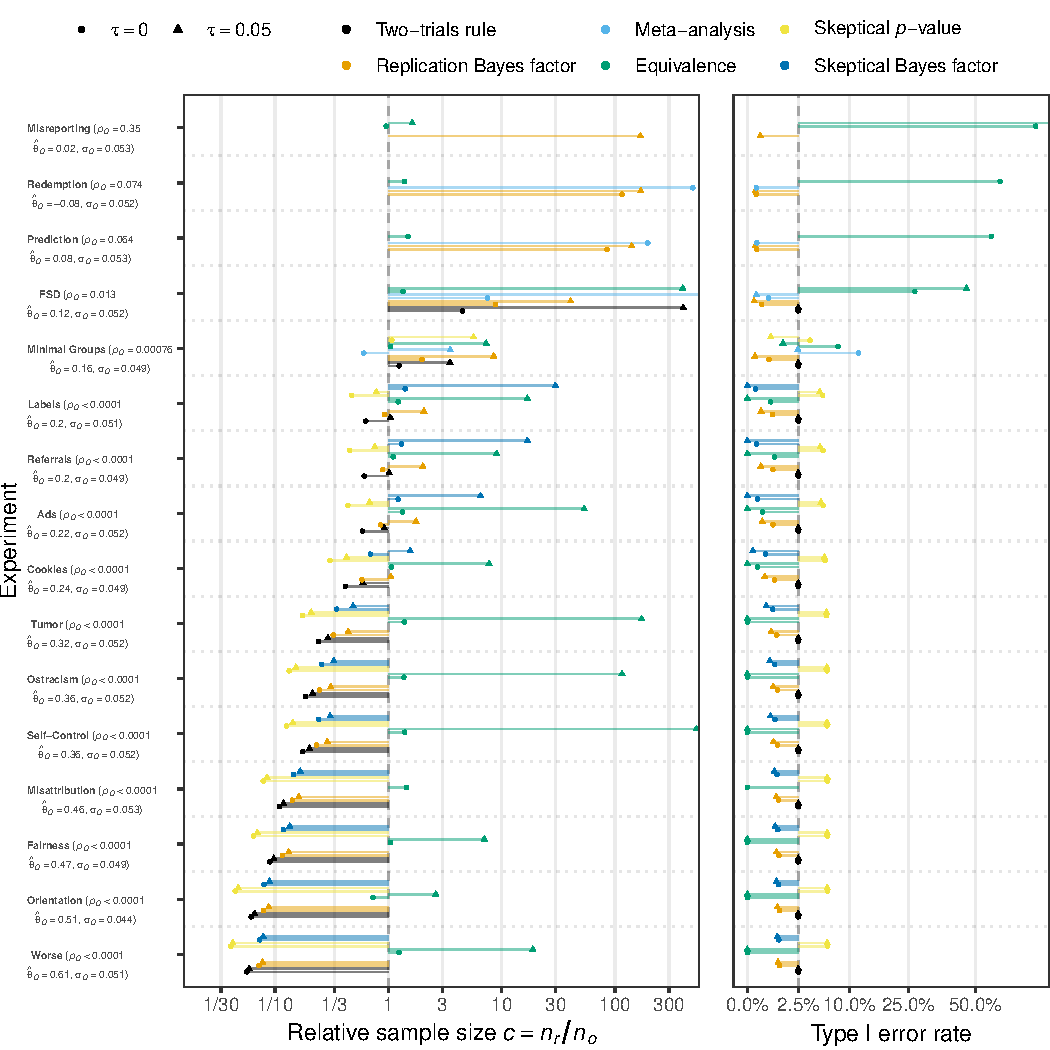
\includegraphics[width=\maxwidth]{images/paper3/sup-ssd-protzko-1}
\end{knitrout}
\caption{The left plot shows the required relative sample size $c = n_r/n_o$ to
  achieve a target probability of replication success of $1 - \beta = 80$\% (if
  possible). Replication success is defined through the two-trials rule at level
  $\alpha = 0.025$, replication Bayes factor at level $\gamma = 1/10$, fixed
  effects-meta analysis at level $\alpha = 0.025^{2}$, effect size equivalence
  at level $\alpha = 0.1$ with margin $\Delta = 0.2$, sceptical $p$-value at
  level $\alpha = 0.062$, and sceptical Bayes factor at level $\gamma = 1/10$
  for data from the replication project by \citet{Protzko2020}. An adaptive
  shrinkage prior is used for the effect size $\theta$ either without
  ($\tau = 0$) or with between-study heterogeneity ($\tau = 0.05$). The right
  plot shows the type I error rate associated with the required sample size.
  Experiments are ordered (top to bottom) by their original one-sided $p$-value
  $p_{o} = 1 - \Phi(|\hat{\theta}_{o}|/\sigma_{o}$).}
\label{fig3sup:ssd-all-shrink}
\end{figure}


\subsection{Sample size determination with adaptive shrinkage prior}
\label{sec3sup:ssdprotzko}
Figure~\ref{fig3sup:ssd-all-shrink} shows sample size determination for all
studies from the \citet{Protzko2020} project as in the main manuscript but using
an ``adaptive shrinkage prior'' for the effect size $\theta$ where the variance
of the shrinkage prior is estimated by empirical Bayes. We see that the required
sample size increases for studies with large $p$-values compared to the analysis
based on a flat prior for $\theta$ as in the main manuscript, whereas it stays
about the same for studies with small $p$-values. This is because studies with
large $p$-values receive more shrinkage.
\end{subappendices}

%% Bibliography
\newpage
\bibliographystyle{apalikedoiurl}
\bibliography{bibliography}
